\section{Introduction}

% Motivate need for new process
The standard method of producing ammonia at industrial scale is through the thermochemical synthesis with the well-known Haber-Bosch process \cite{Schloegl_2003}. This process transformed the global fertilizer industry during the early 1900's, and is a critical enabler of the continued expansion of human population \cite{Smil_1999} -- N-fertilizers are estimated to feed half of the global population \cite{Zhang_2015}. The Haber-Bosch process is an impressive feat of modern chemical engineering, producing 140 million (Fig. \ref{fig:ammonia_prod}) tonnes of ammonia per year at a thermochemical efficiency of up to 70\% \cite{Schloegl_2003,Schiffer_2017}. However, the process also has downsides. The scale of the process leads massive energy consumption of 2.5 exajoule per year, with the hydrogen feedstock typically obtained via the methane reforming reaction \cite{Abbas_2010}, leading to a carbon footprint of 340 million tonnes of CO$_2$ equivalent per year. This is the highest carbon impact of any commodity chemical \cite{Schiffer_2017}. Furthermore, the high temperatures ($\sim$700 K) and pressures ($\sim$100 bar) lead to substantial capital and operational costs. The economies of scale for these costs favor large plants and highly centralized production with $<$100 plants worldwide with an average capacity of 2200 tonnes day$^{-1}$ \cite{McArthur_2017, Bartels}. This is in contrast to the dispersed use of ammonia-based fertilizers globally (Fig. \ref{fig:usemap}), which results in high transportation costs and additional carbon emissions \cite{West_2002}. This is particularly relevant and impactful in remote locations such as in sub-Saharan Africa, where soils are often nutrient limited due to low or no access to fertilizer by smallholder or poor resource farmers \cite{Gilbert_2012, Mueller_2012, VanderVelde2014, Liu2016}, leading to Africa having significantly lower usage of fertilizer compared to other regions (see \ref{fig:ammonia_prod}b). While global hunger has historically decreased with ammonia production, this trend has recently reversed (Fig. \ref{fig:ammonia_prod}a), suggesting that current practices prevent produced ammonia from reaching the agricultural areas where it is most necessary. The opposite problem of over fertilization also has a negative environmental impact in more developed regions due to the periodic application of higher rates of concentrated fertilizers that cause nitrate pollution through leaching into waterways, causing vast ocean ``dead zones'' \cite{Diaz2008, Stevens_2019} as well as high emissions of gaseous nitrous oxide that contribute to climate change. Finally, the intense conditions and reactive nature of concentrated ammonia-based fertilizer lead to safety and national security concerns, as evidenced by explosions at fertilizer plants and the common use of fertilizers in makeshift explosives \cite{Marlair_2005}.

\begin{figure}
    \centering
    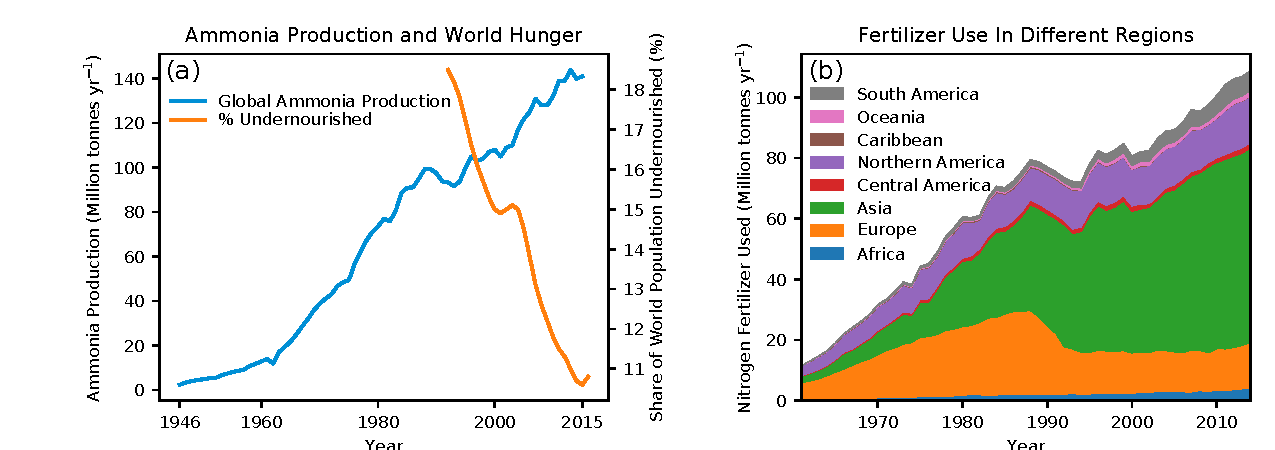
\includegraphics[width=1\textwidth]{Figures/ammonia_production_2.pdf}
    \caption{(a)The worldwide ammonia production each year since 1946 \cite{Kelly_2005} and \% of individuals who are undernourished globally \cite{owidhungerandundernourishment}. (b) the use of nitrogen fertilizer over time denominated by region \cite{owidfertilizerandpesticides}}
    \label{fig:ammonia_prod}
\end{figure}

%\begin{figure}
%    \centering
%    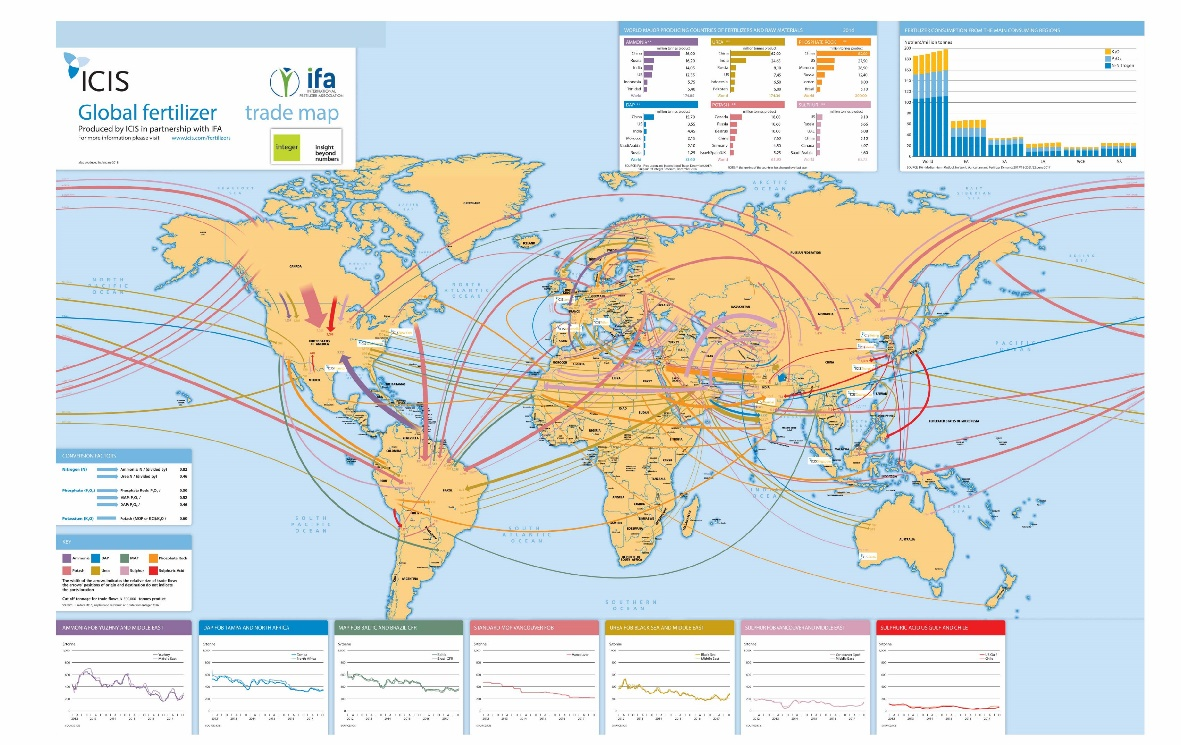
\includegraphics[width=1\textwidth]{Figures/decentralization.jpg}
%    \caption{\hl{placeholder figure for illustration of decentralization. Overlay fertilizer use with locations of ammonia plants. Possibly include solar flux map.}}
%    \label{fig:usemap}
%\end{figure}

%\begin{figure}
%    \centering
%    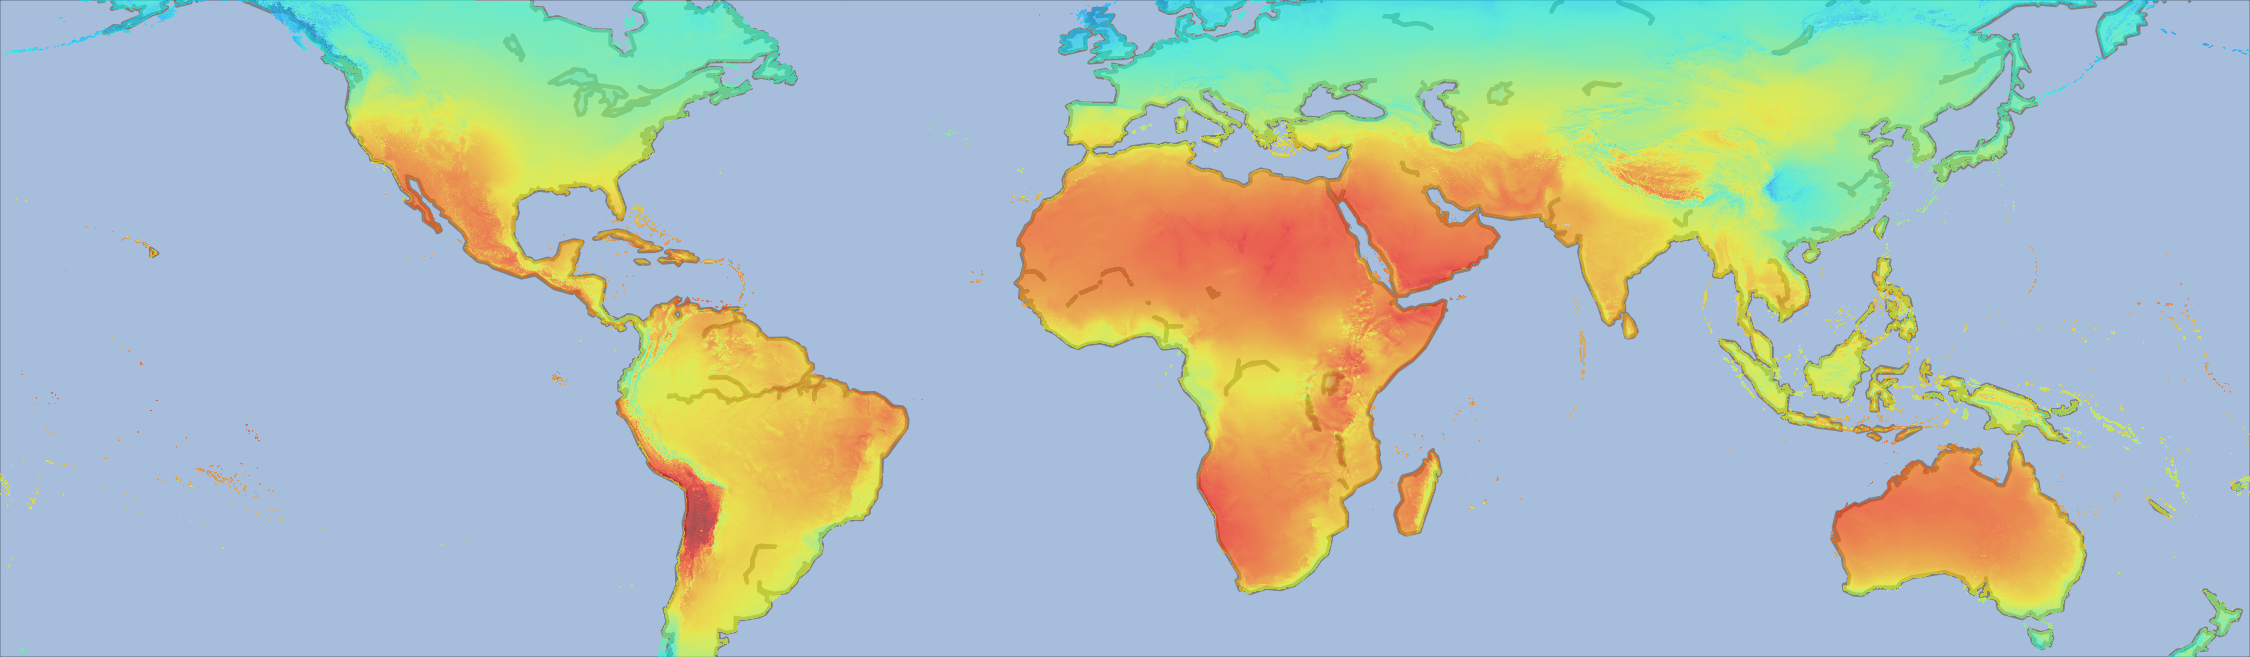
\includegraphics[width=1\textwidth]{Figures/solar_map.png}
    %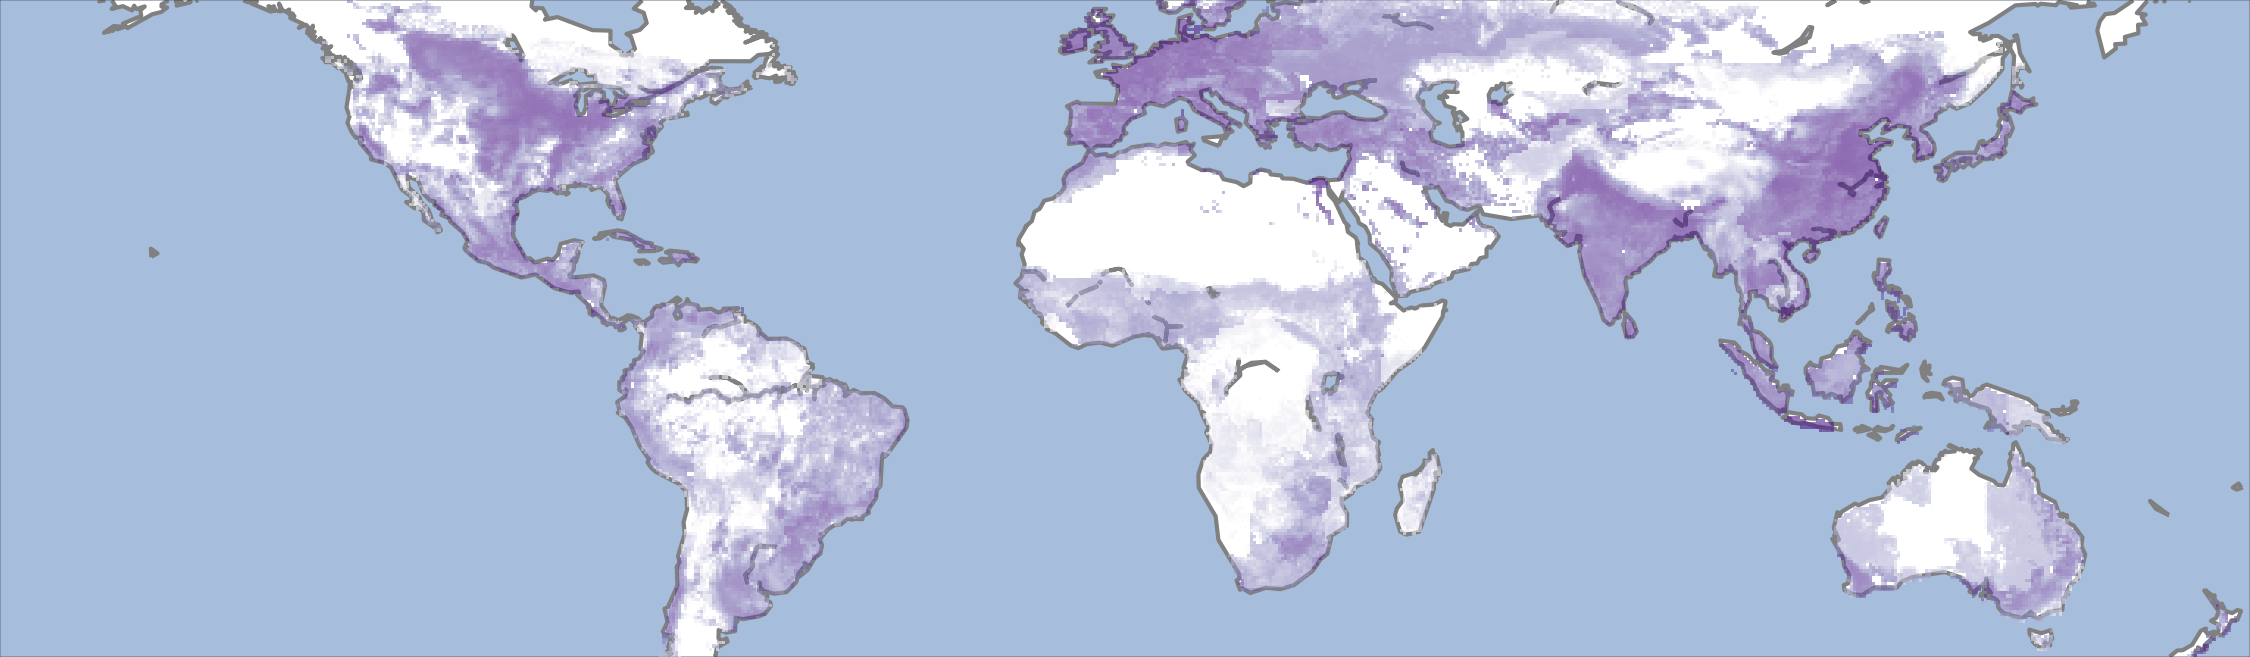
\includegraphics[width=1\textwidth]{Figures/N_fertilizer_map.png}
%    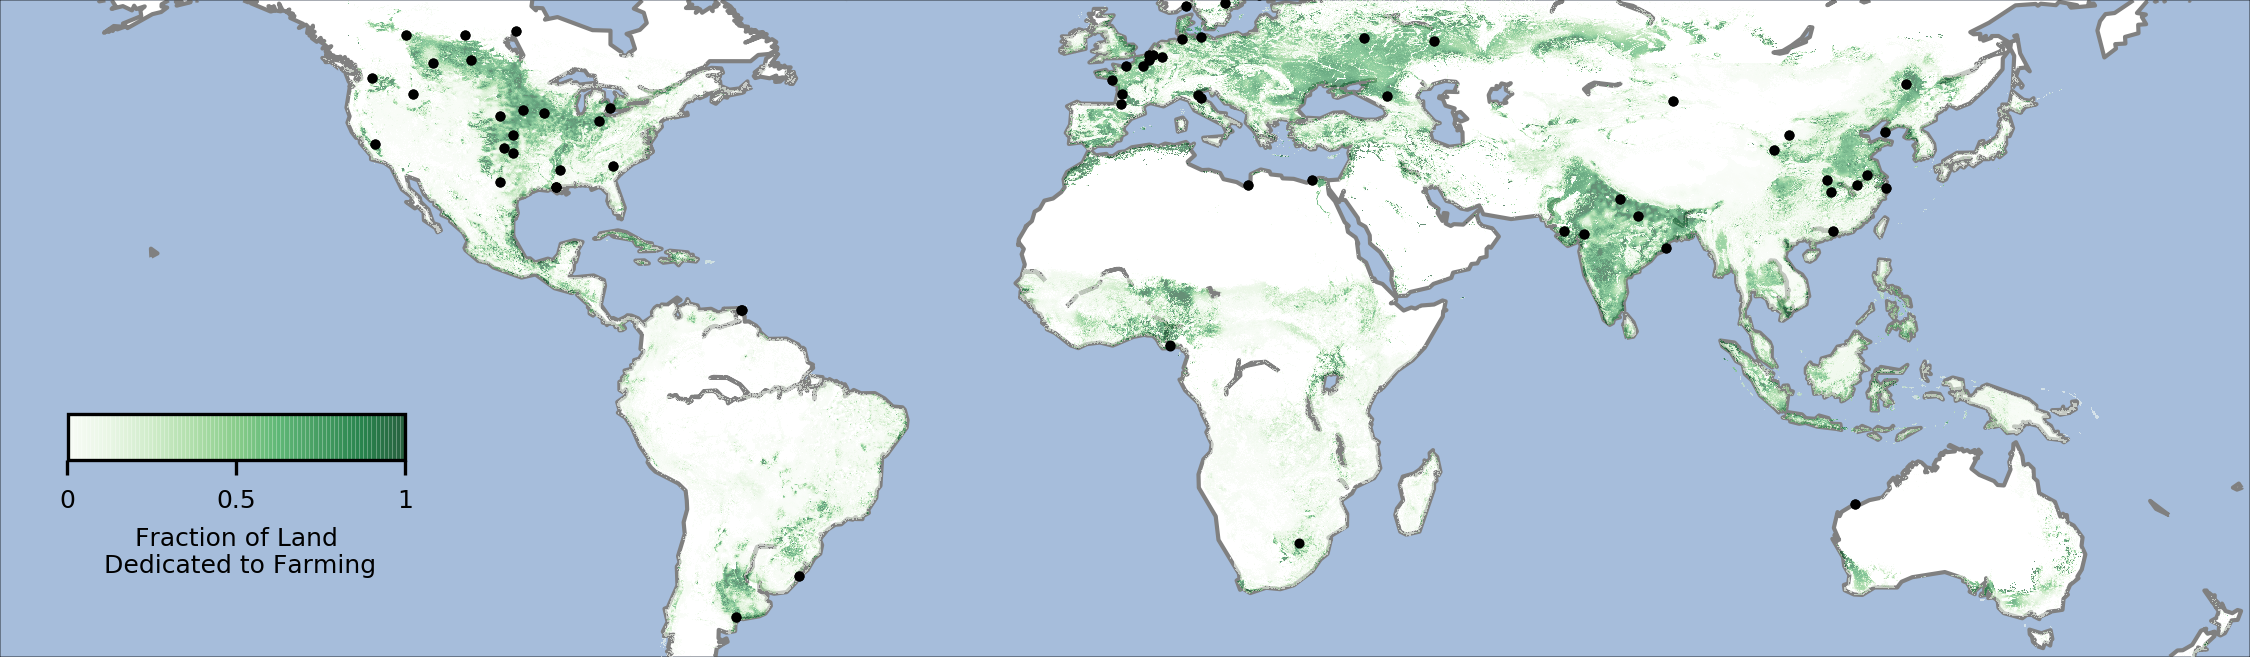
\includegraphics[width=1\textwidth]{Figures/croplands_map.png}
%    \caption{(top) Horizontal solar radiation intensity over the surface of the earth averaged ($kW/m^2$). Solar resource data obtained from the Global Solar Atlas, owned by the World Bank Group and provided by Solargis. (bottom) Percent of land dedicated to crop production (\%), dots represent the locations of Haber Bosch plants. Cropland data from Ramankutty et. al. \cite{Ramankutty_2008, Ramankutty2010} Haber-Bosch plant data from McArthur et. al.\cite{McArthur_2017}}.
%    \label{fig:usemap}
%\end{figure}



%http://sedac.ciesin.columbia.edu/data/sets/browse?facets=theme:agriculture
%http://globalsolaratlas.info/downloads/world

% Motivate solar fertilizers
One possible strategy to overcome these disadvantages of traditional fertilizer is by decentralizing production through the use of solar energy. ``Solar fertilizers'' offer an alternative for local fertilizer production by harnessing solar energy, nitrogen, and water/oxygen from the air to produce low-concentration ammonia- or nitrate-based fertilizers at or near farms where they will be used \cite{Jewess_2016}. This is advantageous since the intermittent solar energy can be directly captured in a storable chemical product that can be utilized near the point of production, avoiding long distance transportation or storage of electrical energy in batteries \cite{MacKay_2013}. This decentralized production will reduce the barrier to adoption of solar fertilizers as compared to solar fuels, since there is no need for retro-fitting the distribution and utilization infrastructure. Solar fertilizers are a special case of ``solar chemicals'' where the close coupling to agriculture provides unique advantages and the product does not compete directly with current ammonia production, but rather reduces the downstream usage of ammonia and N-fertilizers. The economic advantages arise from inexpensive feedstocks (air, water, sunlight) and the elimination of long haul transportation. There is also a societal benefit since solar fertilizers may improve access to fertilizers in remote regions of developing countries. Additionally, the characteristics of fertilizers with low nutrient concentrations may enable novel strategies of nutrient management that can reduce groundwater and atmospheric pollution due to nutrient losses. These advantages reveal significant potential for reducing downstream fertilizer usage, which is linked to energy usage. A recent estimate revealed that even a 10\% reduction in the use of ammonia or urea fertilizers can save around 250 petajoules of energy per year \cite{Levi_2018}. Furthermore, low-concentration fertilizers produced at ambient conditions are inherently safer from the perspective of both process and product handling. Although fertilizer products require a range of macronutrients including N, P, and K, here we focus on N production since nitrogen often the most limiting nutrient in agricultural production\cite{Yousaf2017, VanderVelde2014}.

% Motivate need for collaboration with agriculture/fertilizer
Solar fertilizers hold substantial promise as alternative to traditional fertilizer and for sustainable agriculture, but there are also considerable challenges. One critical challenge is in the development of a viable strategy for efficiently using solar energy to break the strong dinitrogen triple bond at ambient conditions. Nitrogen fixation at ambient conditions is a key objective of chemistry and has been the subject of considerable research in homogeneous catalysis, enzyme catalysis, and bioengineering. Yet, no viable strategies have emerged due to issues with low conversion and/or stability under realistic conditions \cite{Vicente_2017,Bur_n_2017,MacLeod_2013,Foster2018}.
More recently there has been a surge of interest in photo- and electro-catalytic nitrogen fixation by heterogeneous catalysts \cite{Jewess_2016, Medford_2017,Kyriakou_2017,Foster_2018,Chen_2018,Tao_2019,Song_2019,Luo_2018,Wang_2018}. The term photo(electro)chemical is used here to denote various strategies of direct photocatalytic conversion, indirect electrochemical conversion, or a combined photo(electro)chemical approach. These possibilities are particularly interesting from the perspective of solar fertilizers since photo(electro)chemical systems interface well with solar energy, and have the potential to scale relatively easily \cite{Jewess_2016}. Photo(electro)chemical systems have also been the subject of considerable research and progress in the solar fuels community, demonstrating the potential for relatively high energy efficiencies exceeding 10\% \cite{walter_2010, Pinaud_2013,Kondratenko2013,Shaner_2016, Lewis_2016, Montoya_2017}. However, further work is needed to improve the yield and efficiency of photo- and electrochemical nitrogen fixation, and aspects of process design and agronomics have not yet been considered. %In this work we focus on photo(electro)chemical routes to solar fertilizer production and seek to identify targets and strategies for future research.

Solar fertilizers will differ significantly from traditional fertilizers, opening a range of additional agronomic challenges and opportunities. One key difference is that ``solar fertilizers'' are expected to have considerably lower fixed nitrogen concentration. This is related to the fact that most photo(electro)chemical nitrogen fixation processes will have efficiencies far below the 70\% thermochemical efficiency of the Haber-Bosch process \cite{Schloegl_2003, Singh_2017}.
Separating and concentrating the ammonia will require additional steps that add complexity to the process and require additional energy. On the other hand, direct utilization of dilute or low concentration fertilizer will reduce the amount of energy needed for separation/concentration, and may enable more controlled nutrient management in agricultural production\cite{Bar_Yosef_1999,kafkafi2011fertigation}. However, this represents a paradigm shift in agricultural practice, and considerable efforts are needed to understand how dilute solar fertilizers can be sustainably and practically integrated into current agricultural systems. These considerations will also inform the development of the photo(electro)catalytic processes for solar fertilizer production, and hence should be considered in parallel.

%\begin{figure}
%    \centering
%    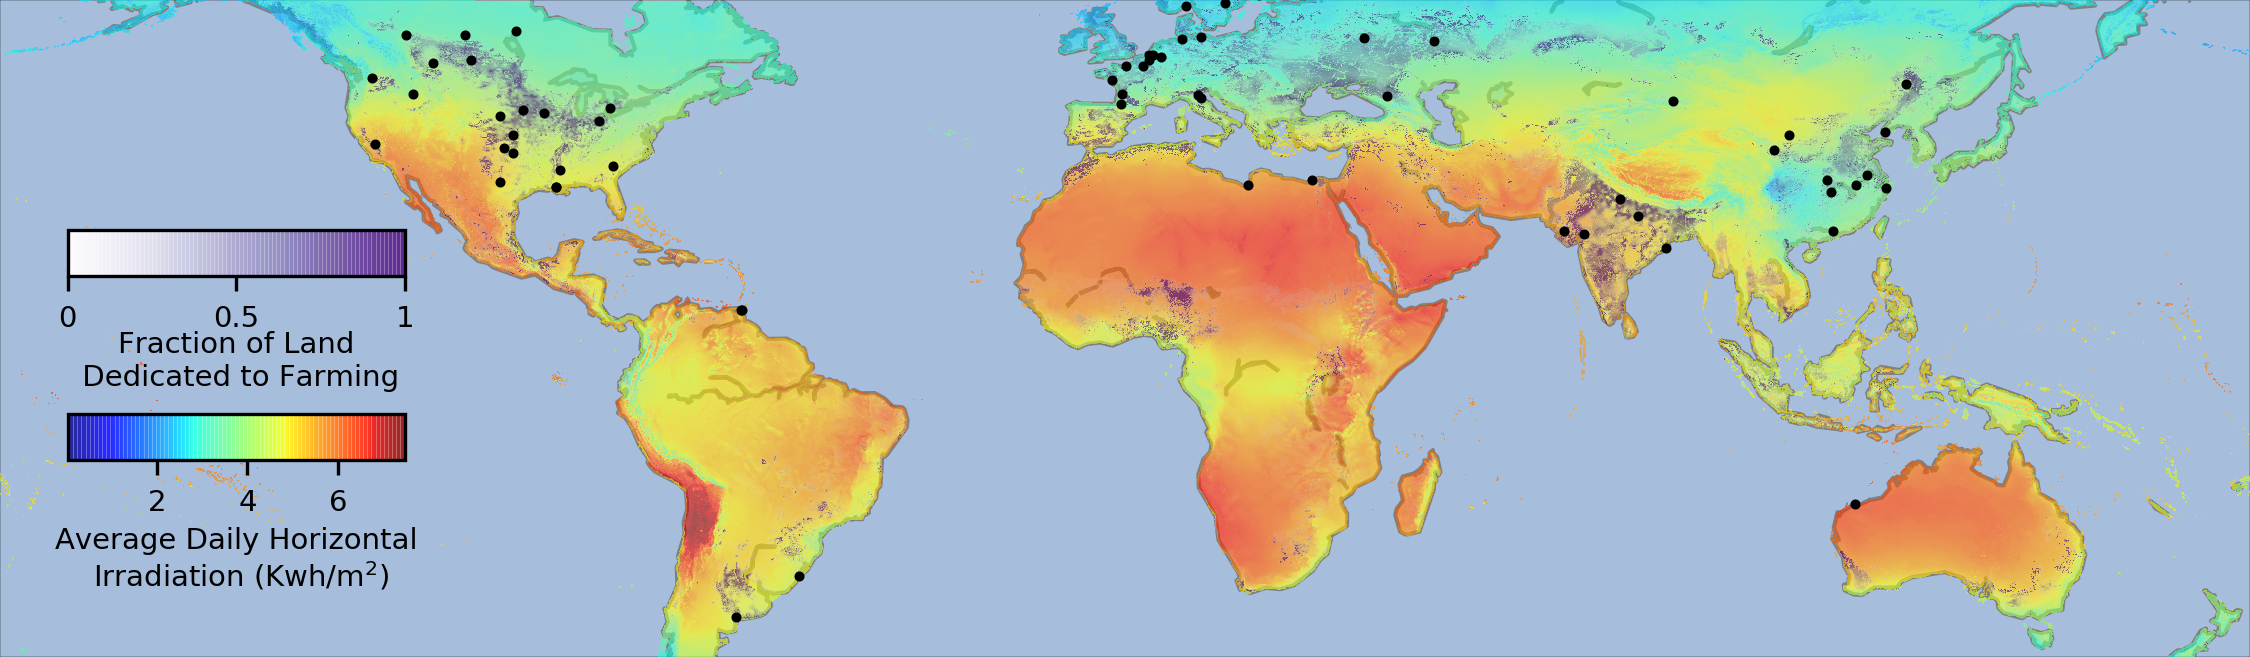
\includegraphics[width=1\textwidth]{Figures/solar_map_w_crop.png}
%    %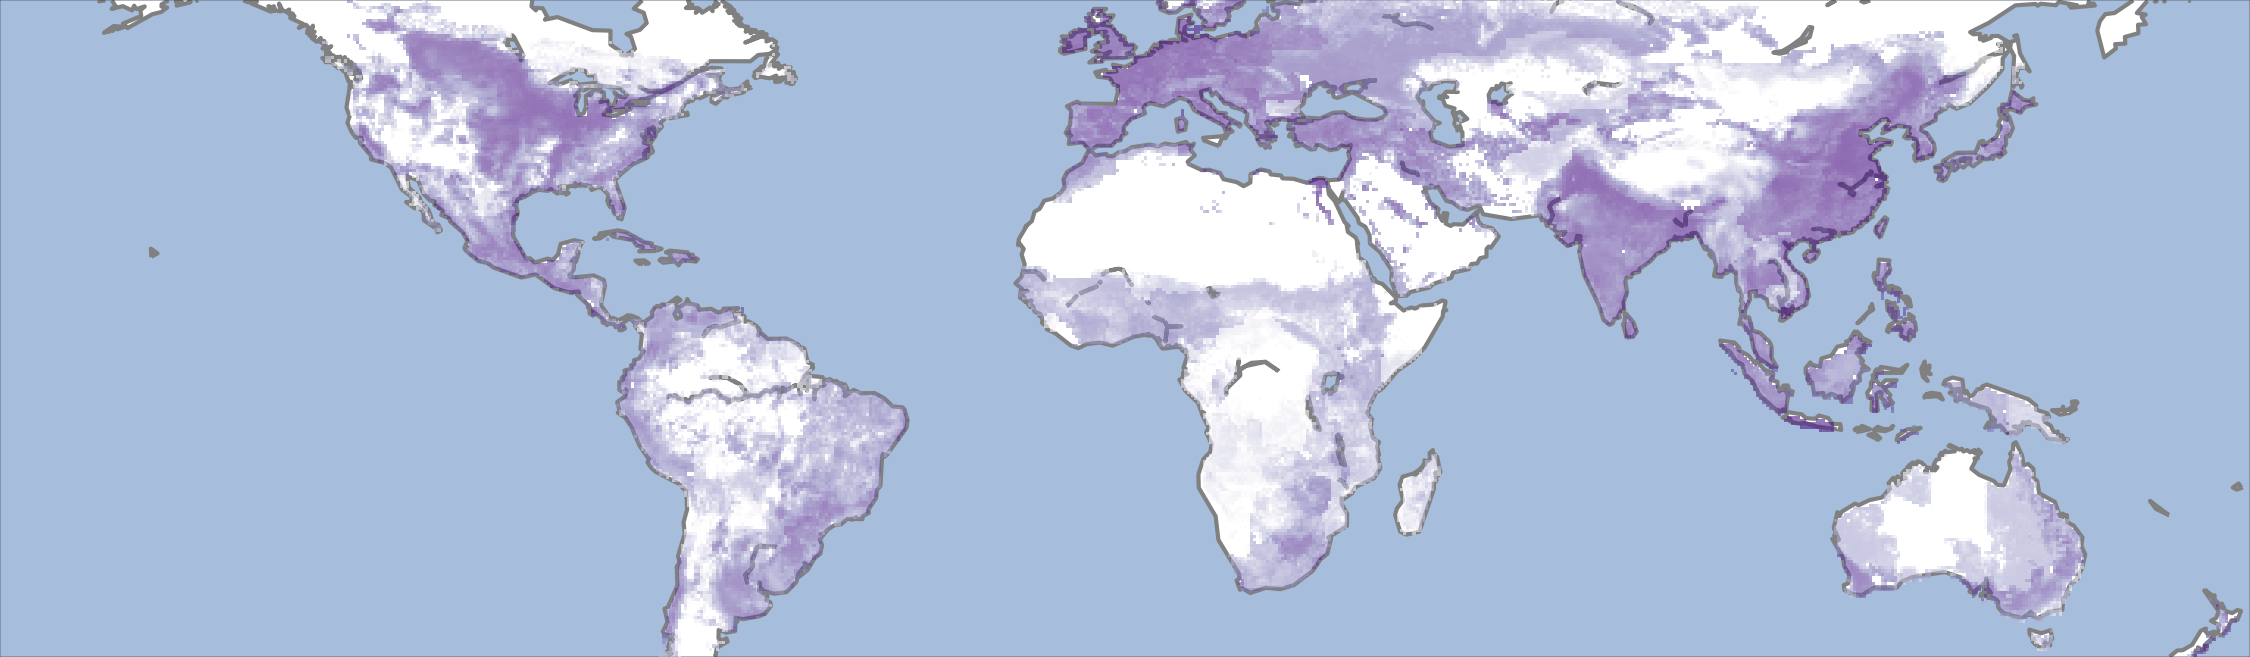
\includegraphics[width=1\textwidth]{Figures/N_fertilizer_map.png}
%    \caption{Average daily horizontal solar radiation intensity over the surface of the earth ($kWh/m^2$).  and fraction of land dedicated to crop production (\%), dots represent the locations of Haber Bosch plants. Solar resource data obtained from the Global Solar Atlas, owned by the World Bank Group and provided by Solargis. Cropland data from Ramankutty et. al. \cite{Ramankutty_2008, Ramankutty2010}. Haber-Bosch plant data from McArthur et. al.\cite{McArthur_2017}}.
%    \label{fig:usemap}
%\end{figure}

\begin{figure}
    \centering
    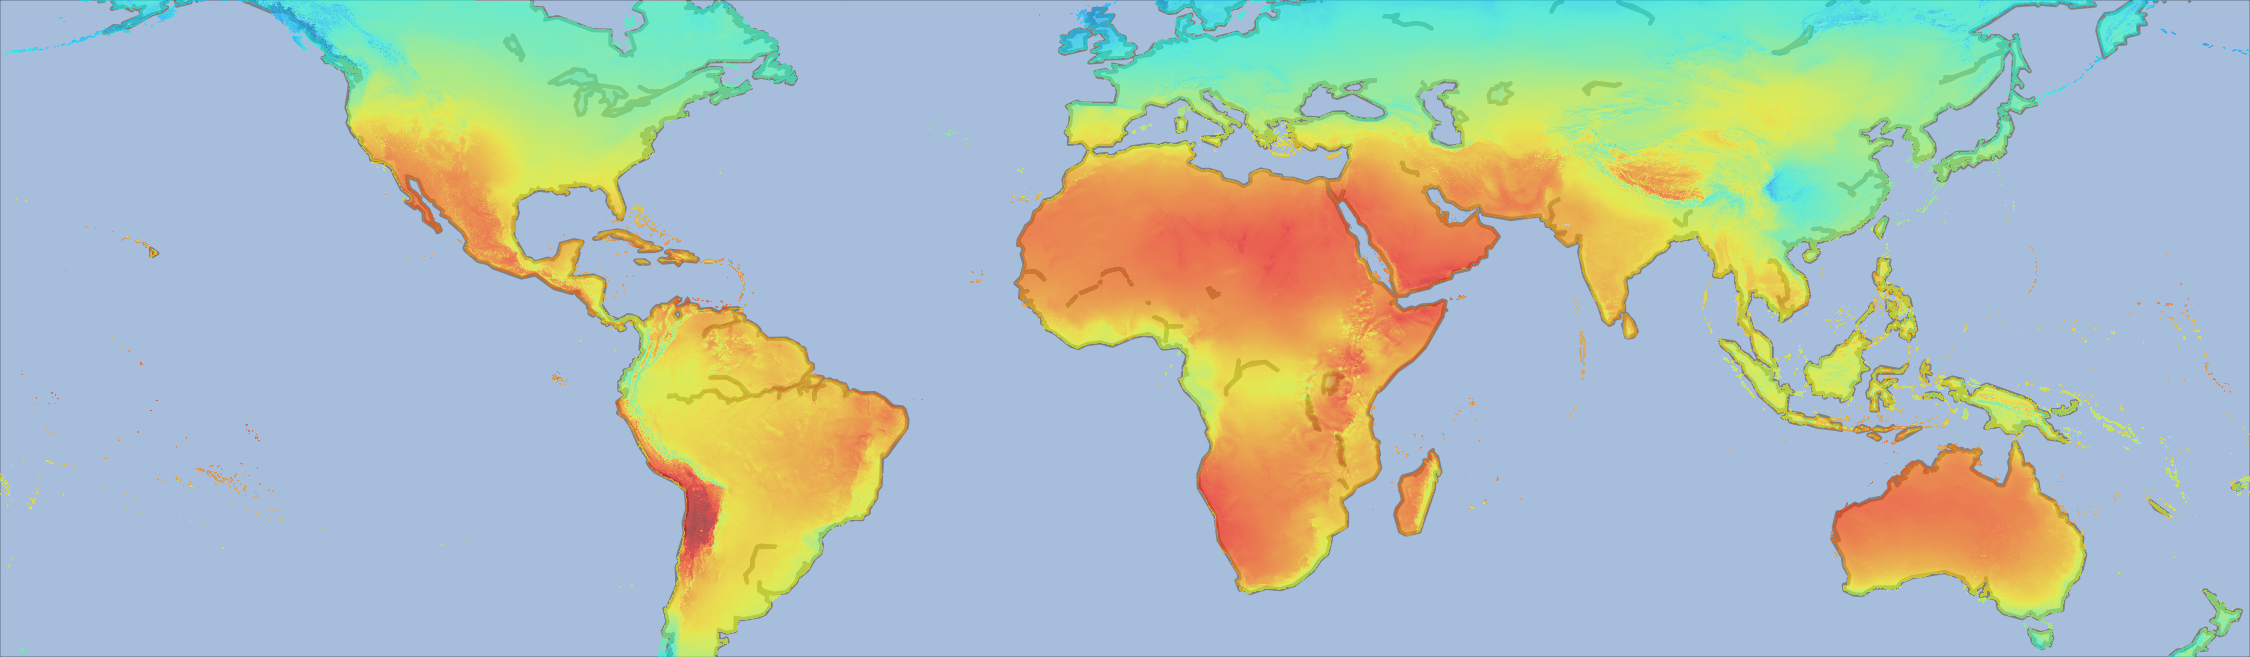
\includegraphics[width=1\textwidth]{Figures/solar_map.png}
    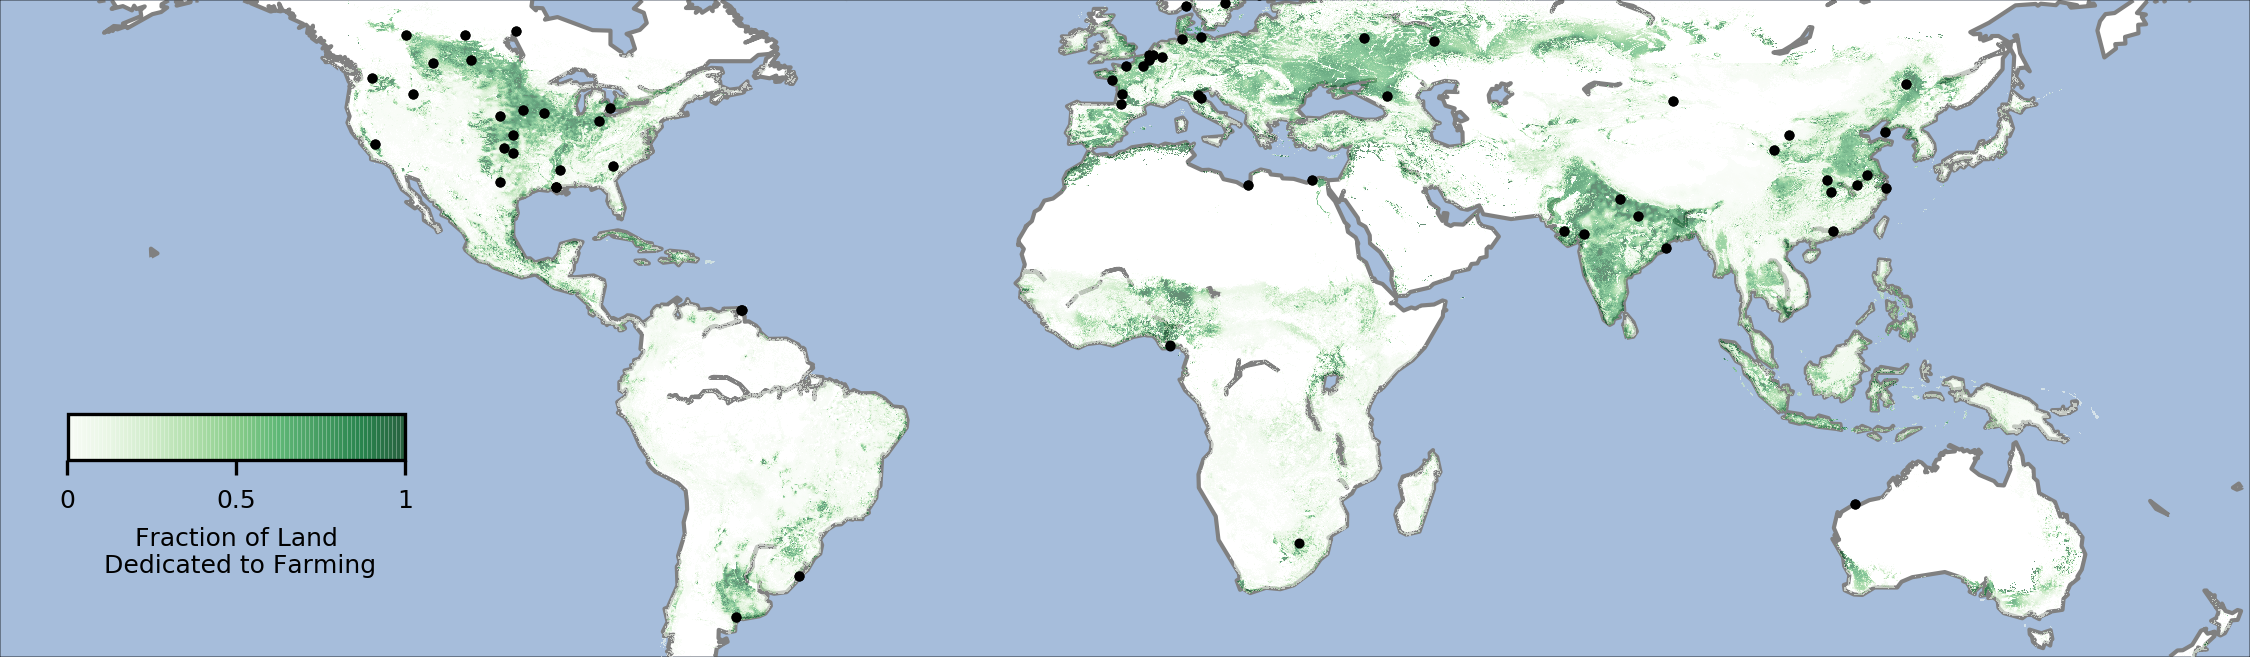
\includegraphics[width=1\textwidth]{Figures/croplands_map.png}
    %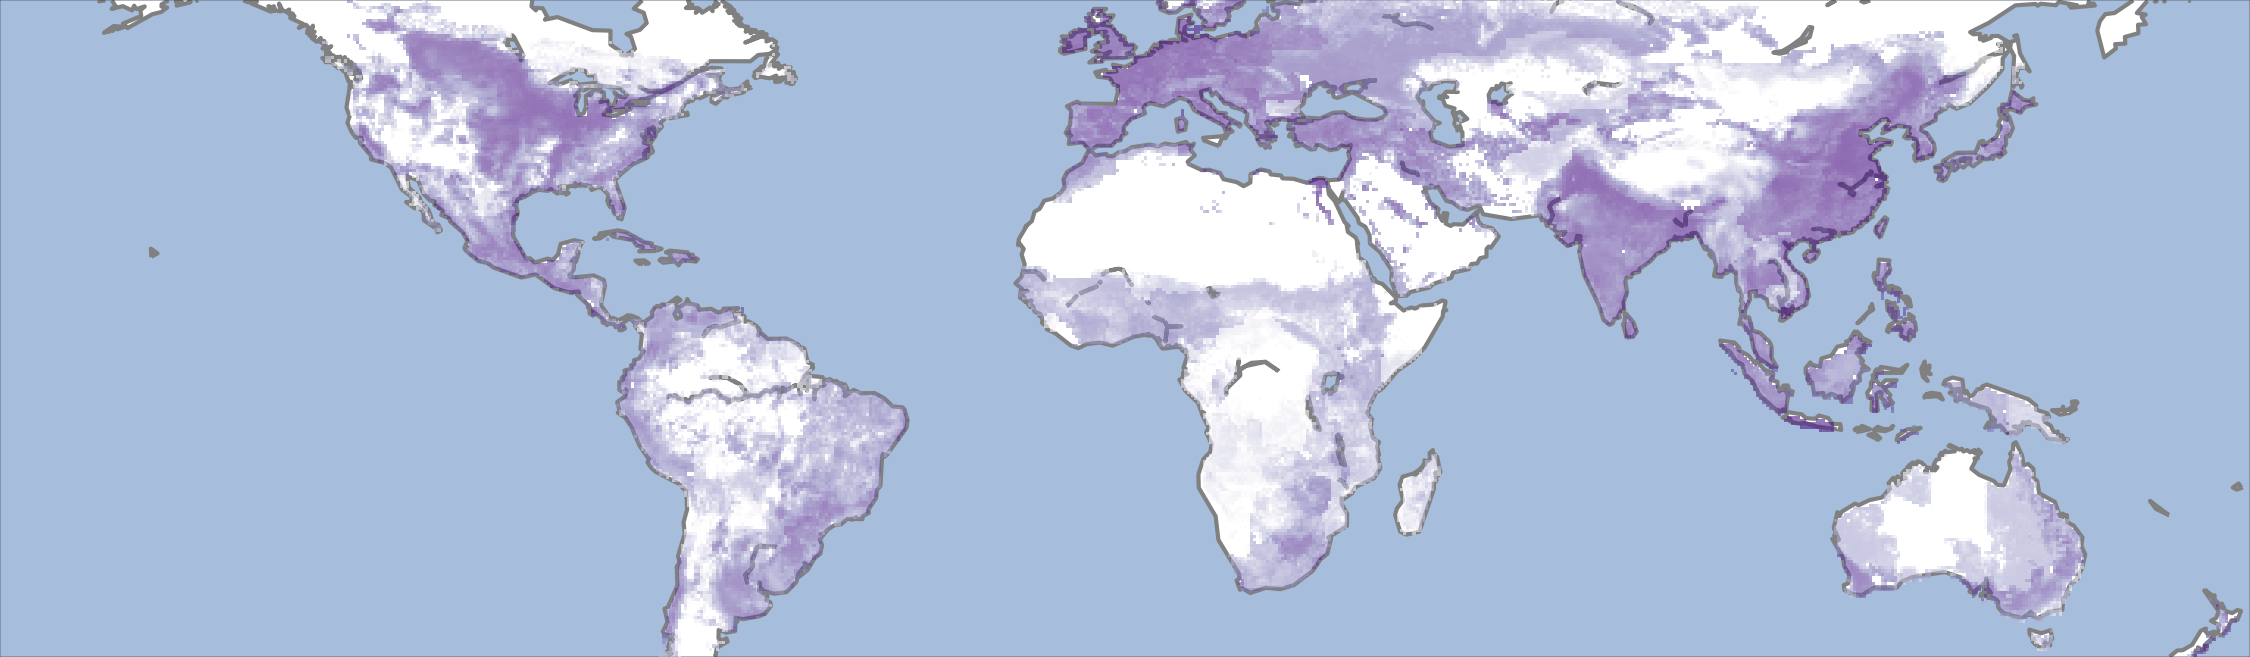
\includegraphics[width=1\textwidth]{Figures/N_fertilizer_map.png}
    \caption{(top) Average daily horizontal solar radiation intensity over the surface of the earth ($W/m^2$). This represents the average flux over a 24 hour period. (bottom) Fraction of land dedicated to crop production (\%), dots represent the locations of Haber Bosch plants. Solar resource data obtained from the Global Solar Atlas, owned by the World Bank Group and provided by Solargis. Cropland data from Ramankutty et. al. \cite{Ramankutty_2008, Ramankutty2010}. Haber-Bosch plant data from McArthur et. al.\cite{McArthur_2017} and Africa Fertilizer \cite{africafertilizer_2018}.} 
    
    
    \label{fig:usemap}
\end{figure}

In this paper we identify key considerations and performance targets for the photo(electro)chemical production of dilute solar fertilizer from the perspectives of agronomics and chemical engineering. Some specific advantages and disadvantages of dilute and decentralized fertilizer production are outlined, and the potential agronomic use cases and impacts are examined. The technical requirements for a photo(electro)chemical reaction/separation process for fertilizer production are considered, and a range of possibilities are introduced. These possible designs are used along with back-of-the-envelope calculations to quantify initial performance targets and limiting cases for catalyst reactivity and suggest specific materials properties and tests that will inform process design. We hope that these considerations will serve as a foundation and guide for future research in the development of photo(electro)chemical processes for solar fertilizer production.

\section{Agronomics of solar fertilizers}

Current fertilizer production relies on the Haber-Bosch process, with highly centralized production and fewer than 100 production plants globally \cite{McArthur_2017} to cater to 1.55 billion hectares of arable land and permanent crops (about 12\% of total land area) \cite{FAOSTAT_2018} and an estimated 500 million farms \cite{FAO_2014,Lowder_2016}. The centralized production is driven primarily by the harsh reaction conditions of the process. The high temperature and particularly the pressure of the process lead to a favorable economy of scale, with a typical capacity scaling exponent of 0.7 \cite{Ullmann_amm_2006, Berthouex_1972}. This incentivizes high-volume production with high capital investment, with the most recent 2200 tonne day$^{-1}$ fertilizer plant having a capital cost of \$1.5 billion \cite{northern_plains_2013}. This leads to long payback periods, and encourages development of production facilities in regions with stable access to feedstock such as natural gas, reliable infrastructure, stable governance, and sophisticated financial systems \cite{McArthur_2017} as indicated by the presence of ammonia production primarily in developed regions (Fig. \ref{fig:usemap}). The resulting fertilizer products with high nutrient concentration must be transported to globally dispersed agricultural production centers. 

Fertilizer use in developing countries has been encouraged due to a significant depletion in soil nutrients. However, for the use of fertilizers to be economically viable and sustainable, they must produce a significant increase in yield. This is typically quantified by the ``value-cost ratio'' (VCR), which in this case is the ratio of crop output value to fertilizer input cost. As a rule-of-thumb, farmers will invest and use fertilizer if the VCR is greater than $\sim$2, indicating that for every dollar invested in fertilizer, output revenues will repay the invested dollar plus an additional dollar, for a 100\% return on investment. As shown in Fig. \ref{fig:vcr} for selected crops the VCR is generally increased as the price of fertilizer decreases \cite{sommer_2013}; however, the prospect of much lower fertilizer prices would clearly incentivize fertilizer use by increasing the VCR, assuming constant or no downward changes in agricultural output prices. It is important that these economic incentives hold for small ($<$ 1 ha) farms, since $>$70\% of farms globally are small (Fig. \ref{fig:vcr}b), and the proportion is higher in developing countries \cite{Lowder_2016}. This section briefly explores the implications of the centralized Haber-Bosch process on the economics of fertilizer production, and explores the potential impact and challenges of decentralized production of dilute fertilizers in both developed and developing regions.
\begin{figure}
    \centering
    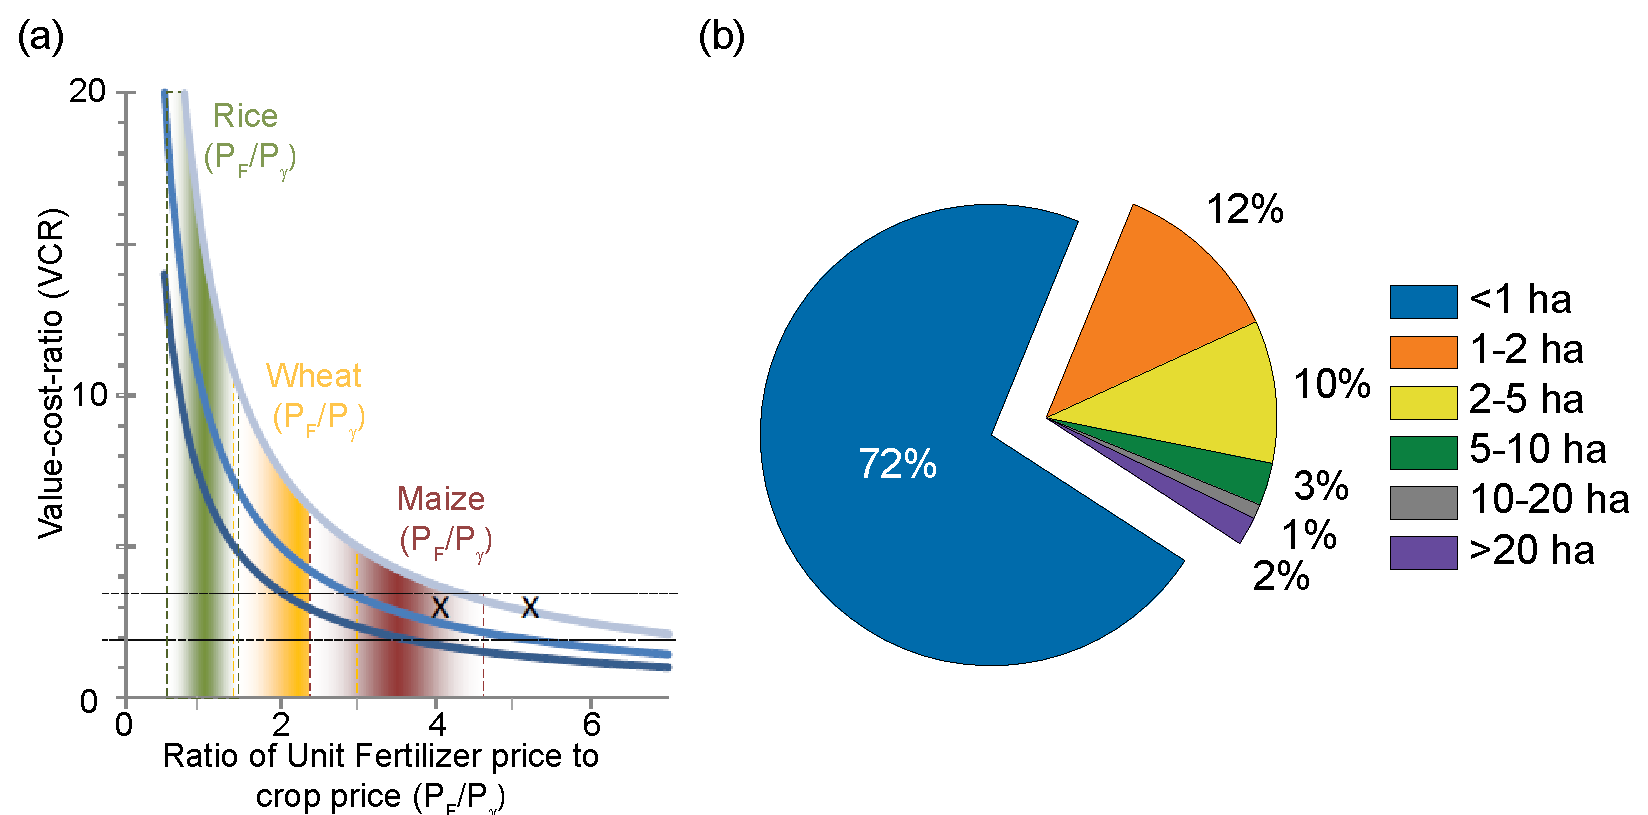
\includegraphics[width=.8\textwidth]{Figures/value_cost_ratio_farm_size.pdf}
    \caption{(a) Value-cost ratio (VCR) in response to the ratio of unit fertilizer price to unit crop price (PF/PY) for
three different levels of fertilizer response (kg yield [Y] per kg Fertilizer [F]; blue curves) \cite{sommer_2013} (reproduced from \cite{Lowder_2016}) and (b) proportions of farms with various sizes.}
    \label{fig:vcr}
\end{figure}

\subsection{Decentralization of fertilizer production}
\label{sec:decentralized}

There are a continuum of options for moving from the current highly centralized fertilizer production toward smaller-scale distributed production. In this section we briefly explore the general economic factors that favor decentralized production and subsequently consider three possible specific scenarios along the continuum of decentralized fertilizer production.
The three scenarios (see Figure \ref{fig:scenarios}) presented here are (1) inexpensive, robust solar fertilizer production at the scale of small farms in remote and undeveloped regions (2) solar fertilizer production integrated with existing infrastructure on larger farms in developed regions, and (3) high-tech solar fertilizer production coupled with production and distribution infrastructure of existing or emerging agricultural products. These scenarios present exciting opportunities to develop scalable decentralized solar fertilizer technologies with the potential for substantial positive impact on society, energy, and the environment.

\begin{figure}
    \centering
    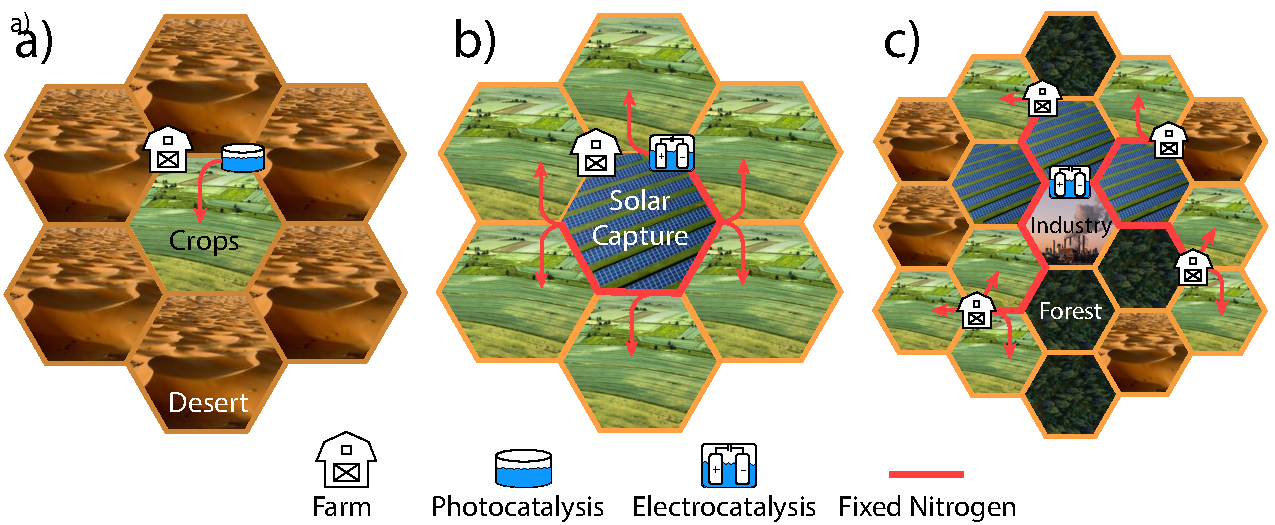
\includegraphics[width=\textwidth]{Figures/solar_fertilizer_scenarios.pdf}
    \caption{The three proposed scenarios for solar ferilizer a) inepensive farm scale production using photocatalysis b) solar ferilizer production integrated with larger farms using electrocatalysis c) high-tech solar fertilization production coupled with distribution infrastructure using electrocatalysis}
    \label{fig:scenarios}
\end{figure}

From a simplistic and practical perspective the major components of fertilizer retail cost can be broken down into production, transportation, and storage costs. The production cost of fertilizer is controlled primarily by the cost of its feedstock, the natural gas used as a source of hydrogen for the Haber-Bosch process and hence, varies with geographic, economic, and geopolitical factors \cite{Huang2007,Etienne2016}. 
This leads to variable and uncertain cost of fertilizers and presents challenges in agricultural planning \cite{Etienne2016}. Furthermore, the cost of transportation depends strongly on the location and transport mode available (barge, rail, trucks, pipeline). Barge, pipeline, and rail transport are normally used for long-distance anhydrous ammonia transportation, while trucks are preferred for shorter distances. Distance, location of plant site relative to the agricultural area, availability of transportation equipment, and relative cost of available carriers are the major governing factors for selection of a typical anhydrous ammonia transportation system. International shipping of ammonia between the United States and Western Europe costs on the order of \$ 35 per tonne \cite{ammonia_encyclopedia}. Typical costs reported in the United States for long distance (greater than 1600 km) by pipeline, barge, and rail transport are \$0.0153, \$0.0161 and \$0.0215 per tonne per kilometer, respectively \cite{ammonia_encyclopedia}.  Short truck transportation costs are expected to be much higher. For distances of the order of 100 km, typical reported costs are \$0.0365 per ton per kilometer \cite{ammonia_encyclopedia}. Additionally, storage costs must be considered due to the seasonal consumption of ammonia caused by agriculture's cyclic nature. It has been reported that roughly 75\% of the fertilizer production is sold in the spring during the planting season \cite{ammonia_encyclopedia}. To reduce storage costs resulting from this cyclic consumption pattern, large refrigerated anhydrous ammonia storage vessels are used, which add another \$11-80 per tonne to ammonia cost \cite{IFDC_1998,ammonia_encyclopedia}. Thus, the freight costs can account for more than half of the retail cost of ammonia in some countries.
The hazardous nature of ammonia also leads to challenges with transportation and storage, particularly in regions with poor infrastructure \cite{Etienne2016}. 

%\begin{figure}
%    \centering
%    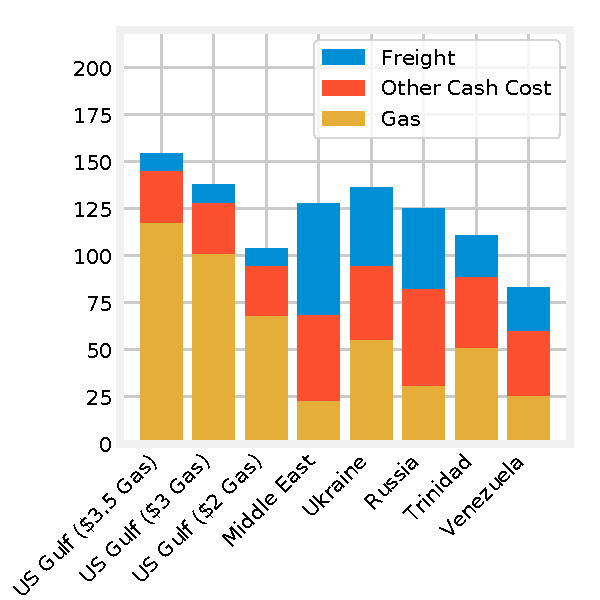
\includegraphics[width=0.5\textwidth]{Figures/Cost_By_location.pdf}
%    \caption{The price of ammonia in units of \$US MMBTU$^{-1}$ in different regions broken down by the price contribution due to transport, cash cost, and natural gas. \st{gas refers to the price of natural gas in \$US MMBTU$^{-1}$}. Data from Maxwell et. al.\cite{maxwell2004synthetic}. \hl{It would be great to have a similar figure with cost breakdown by production/transportation/storage, ideally with numbers from some African countries included.} }
%    \label{fig:relative_costs}
%\end{figure}

\begin{figure}
    \centering
    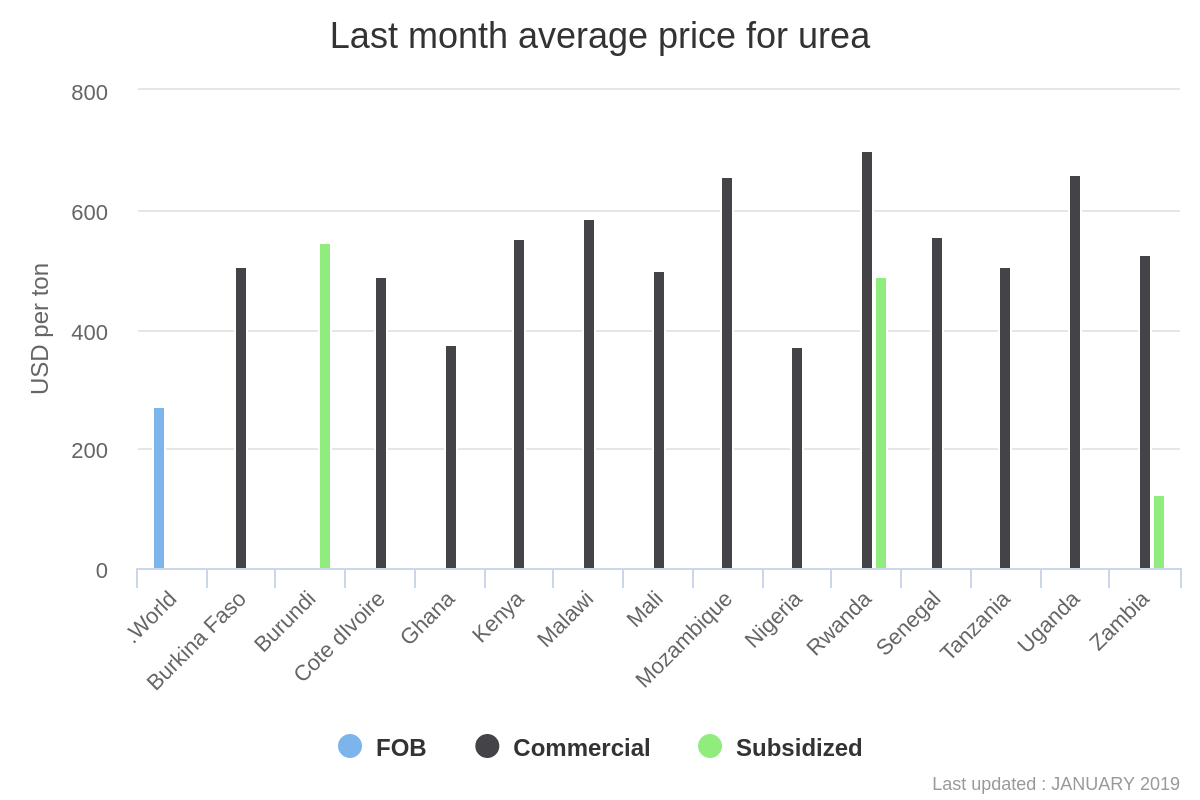
\includegraphics[width=0.7\textwidth]{Figures/africa_costs.png}
    \caption{Overview of current (2019) commercial and subsidized costs of fertilizers in various African countries compared to the international free on board (FOB) cost \cite{africafertilizer_2018}.}
    \label{fig:africa_costs}
\end{figure}

The production, transportation, and storage costs are the main components of fertilizer price, but the overall cost is not directly derived from these categories. For example, as shown in Fig. \ref{fig:cost_pies} the price of fertilizer in Thailand (\$ 287 t$^{-1}$) is roughly half the price of fertilizer in Mali (\$ 509 t$^{-1}$), but this difference cannot be attributed directly to any single category \cite{Wanzala2013}. This discrepancy is largely due to the economies of scale and to other factors that affect the efficiency of fertilizer procurement and distribution. Developing nations in Africa are often purchasing smaller quantities of fertilizer from the international market, limiting their ability to bargain for lower wholesale prices and leading to prices that are generally much higher in African countries (Fig. \ref{fig:africa_costs}) \cite{Wanzala2013}. Larger agricultural markets such as in Asia can more effectively negotiate and distribute fixed costs of transportation across more units of fertilizer, reflected in lower prices of fertilizer at retail. This scale-up is not possible in less developed markets for a variety of reasons including port capacity and poor transportation infrastructure \cite{Chianu_2011}. Political instability often compounds this problem by causing existing infrastructure to deteriorate due to lack of investment \cite{IFDC_2012, IFDC_2012_2, IFDC_2012_3}. Road systems in these regions are often not well maintained or regulated, leading to worse connectivity and excessive wear and tear on transportation equipment. Less developed markets are also subject to more uncertain demand owing to lack of access to finance by smallholder farmers and unpredictable implementation of government subsidies \cite{Chianu_2011,IFDC_2012, IFDC_2011, IFDC_2012_2, IFDC_2012_3}. These subsidies can be critical for making fertilizer more affordable to smallholder and resource poor farmers  (Fig. \ref{fig:africa_costs}) and removing or reducing subsidies can considerably reduce the amount of fertilizer procured and supplied by private importers. For example, removal of fertilizer subsidies in Ghana in 2014 reduced imports by about 50\%, and most of the product that was imported was provided to commercial operations rather than smallholder farms \cite{IFDC_2018}. Overall, these factors lead to a perverse situation in which fertilizers are most expensive in the poorest places where the need is greatest. This is a key factor in the distressing fact that despite the tremendous technological developments of the recent decades and ever-increasing ammonia production, world hunger is has stopped declining and is currently increasing (Fig. \ref{fig:ammonia_prod}) with over 800 million people suffering from undernourishment as of 2016 \cite{FAO_2017}. Notably, many of these economic and geopolitical factors could be alleviated by decentralized production of dilute fertilizers with low capital input from solar/renewable resources. Reducing or eliminating the dependence on natural gas would reduce volatility in fertilizer production costs and prices \cite{Etienne2016}, while producing fertilizer at or near the point of use would reduce transportation costs and perhaps eliminate the cost dependence on economies of scale  \cite{IFDC_1998}. Furthermore, local production would improve certainty in fertilizer availability, reduce the influence on price of external factors such as feedstock price volatility and tariffs, and eliminate the needs for subsidies and their burden on governments’ budgets. Considering that agricultural production is directly linked to general economic prosperity, local fertilizer manufacturing industries in developing countries could spur substantial economic growth \cite{McArthur_2017}.




\begin{figure}
    \centering
    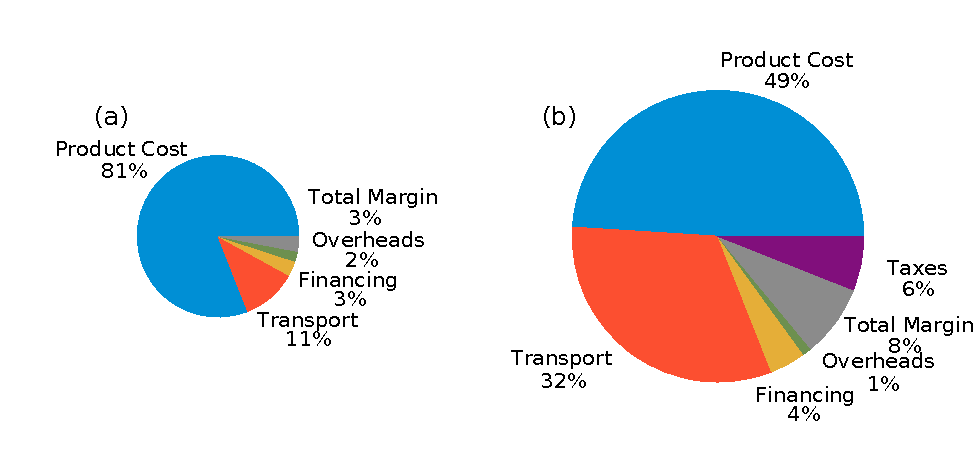
\includegraphics[width=1\textwidth]{Figures/Cost_Breakdown_2.pdf}
    \caption{The price breakdown for fertilizer in (a) Thailand and (b) Mali for the year 2013. Relative areas reflect the ratio of costs in the two countries (\$282 in Thailand and  \$509 in Mali) \cite{Wanzala2013}}
    \label{fig:cost_pies}
\end{figure}



%\begin{figure}
 %   \centering
 %   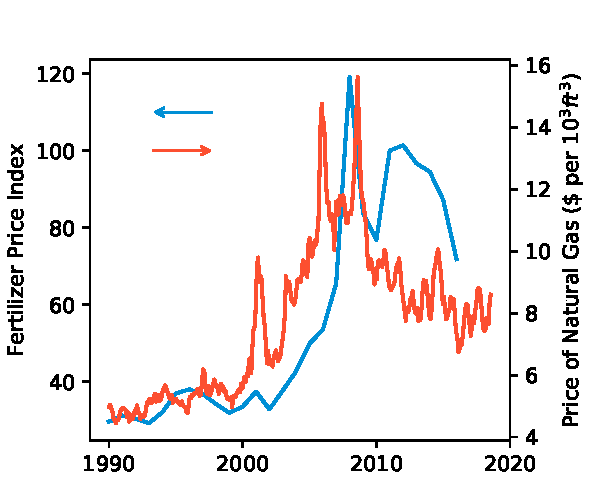
\includegraphics[width=0.7\textwidth]{Figures/gas_vs_fert.pdf}
 %   \caption{The cost of natural gas paid by industrial consumers in the United States and the price index of fertilizer between over time (www.eia.gov and usda.gov)}
%    \label{fig:gas_vs_fert}
%\end{figure}

%The concept of decentralization is difficult to quantify in general \cite{Schneider_2003}, but in this context we propose the decentralization should scale directly with the total number of fertilizer production facilities. It is useful to examine order-of-magnitude estimates of these quantities to assess the prospects of decentralization. A recent report identified a total of 63 major fertilizer production facilities based on data from the 10 largest producers of ammonia-based fertilizers \cite{McArthur_2017}. While this list may be incomplete, it is expected to be on the correct order of magnitude. A typical 1000 tpd ammonia plant can meet the ammonia requirements of many small countries. At a medium application rate of 40 kg N/ha, a typical ammonia plant can fertilize 7.5 million hectares of land. Fertilizer production on this scale is not available in many developing countries; logistics, economic and political issues constrain construction of large scale ammonia plants in such regions.\cite{IFDC_1998} 
%For landlocked countries that are located at a long distance from the ports, the freight cost doubles or even triples the cost of ammonia-based products, and thus limits consumption.

%This should be normalized by the total agricultural output, which we propose can be estimated by the total number of farms or the total amount of arable land. Both numbers are difficult to know exactly, but a 2014 report estimated the total number of farms to be in excess of 570 million with a total area of around 4.9 billion hectares (another FAO document said 1.5 billion ha) as of 2010 \cite{FAO_2014,Lowder_2016}. This indicates that a single ammonia-based fertilizer plant serves on the order of 10 million farms, or 100 million \hl{(24 million)} hectares of arable land (see Figure \ref{fig:map}) \hl{We need to refine these estimates and ensure that the 4.9 billion number does not include grazing land. The map is based off the smaller number of 24 million based on this source: https://ourworldindata.org/yields-and-land-use-in-agriculture.}.
%\begin{figure}
%    \centering
%    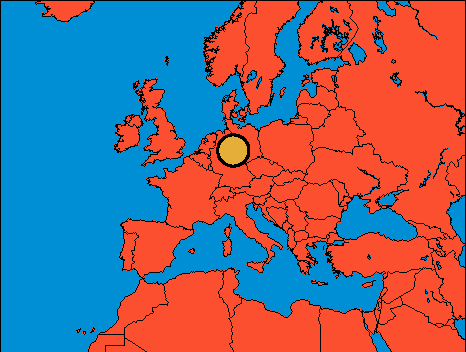
\includegraphics{Figures/approx_size.pdf}
%    \caption{The approximate area of land fertilized by an average single Haber-Bosch plant based on rough estimates above. \hl{Revise as needed based on data estimates.}}
%    \label{fig:map}
%\end{figure}

The most extreme small-scale alternative would be fully decentralized farm-scale fertilizer production (Fig. \ref{fig:scenarios}a), which would have the largest socio-economic and agricultural impact if deployed in low-income countries where access to fertilizer is limited. There is a large range of farm sizes, but most farms in low-income countries are $<$1 ha (Fig. \ref{fig:vcr}b)\cite{Lowder_2016} . With over 70\% of farms being classified as small holdings, a market push toward decentralization could aid a significant portion of the agricultural market. Fertilizer production at the scale of small farms would  correspond to roughly 1 fertilizer production facility per ha, an increase of $\sim$ 7 orders of magnitude in the total number of fertilizer production facilities. Naturally, this would correspond to proportional decrease in the scale of production per facility.
The required nutrient load varies considerably from $\sim$20 - 200 kg-N per hectare depending on crop and region, but we adopt 100 kg-N per hectare per year as a convenient representative nutrient load \cite{Medford_2017}, which can be used to obtain rough estimates of cost and efficiency. For example, the annual budget for on-site fertilizer production can be estimated based on the cost of fertilizer per country. The estimated average cost of supplying urea at retail point in Ghana under open market conditions during 2018 was \$394 per tonne, or \$857 per tonne of nutrient N (urea is nutrient 46\% N by weight) \cite{africa_fert_2017}.
 This corresponds to an expected annual N nutrient fertilizer budget on the order of \$ 86 per hectare per year. This modest number suggests that decentralized fertilizer production at the scale of small farms must have very low capital and operating costs, even in countries where the cost of fertilizer is very high. Furthermore, the process must be sufficiently robust that specialized personnel are not needed for operation or maintenance of production, and additional constraints such as water usage and fertilization infrastructure (e.g. irrigation) must be considered. Strategies of ``frugal innovation'' \cite{Weyrauch_2016} can help address these challenges, and the successful development and deployment of solar energy technology to disinfect water through photochemistry and photocatalysis provides a promising precedent for this approach \cite{Lonnen_2005, McGuigan_2012}.
 %However, the current economic situation in many developing countries leads farmers to use little to no fertilizers \needcite, indicating that even the production of an inferior fertilizer product can impact agricultural output if the cost is sufficiently low and infrastructural requirements are minimal.
 This suggests that the development of inexpensive and robust processes for producing solar fertilizer at the scale of small farms in the developing world may be a viable strategy.
 
An alternative approach to farm-scale production is to target larger farms ($\gtrapprox$ 100 ha), particularly those which are already using irrigation systems that can be directly utilized for delivery of dilute aqueous fertilizer (Fig. \ref{fig:scenarios}b). While these very large farms account for less than 2\% of farm holdings (Fig. \ref{fig:vcr}b), they account for over 45\% of the agricultural land area, and are more common in developed countries \cite{Lowder_2016}. This scenario presents an economic challenge for decentralized N fertilizer production since they will compete directly with traditional fertilizer. For example, the cost of urea in the United States is approximately \$550 per tonne N as of 2018 \cite{Argus_Feb}, though there is significant fluctuation. This is compounded by the larger capacity of the farms, and the typically heavier fertilization in developed countries. Assuming a nutrient load of $\sim$ 100 kg of nutrient per hectare per year for a large 100 ha farm leads to an approximate annual fertilizer budget of $\sim$ \$5,500 per farm (\$55 per ha). This number is relatively modest, but there are additional incentives for larger farms to invest in decentralized fertilization. These larger farms require larger capital investment, and the reduced volatility in price for fertilizers produced on site would improve the predictability of returns. The integration of on-site solar fertilizers with existing irrigation infrastructure may reduce the costs associated with delivering fertilizer to crops, or enable more efficient fertilizer utilization, as discussed further in Sec. \ref{sec:dilute}. There are also challenges for scaling solar fertilizers to larger farms. Solar fertilizer production will require a higher level of technological sophistication, particularly if electrochemical technologies are employed. These approaches will require installation, maintenance, and potentially operation by experts. It is unlikely that a full-time employee could be dedicated to fertilizer production, even at very large farms of $\sim$1,000 ha. Nonetheless, periodic access to experts for installation and maintenance is not an issue in developed regions. Numerous industries such as solar capture and heating ventilation and air conditioning (HVAC) operate on similar business models. This suggests that solar fertilizers are potentially viable for farm-scale production in developed areas as long as they can be operated with only periodic maintenance.

A third scenario is the production of solar fertilizer at a regional, semi-centralized multi-farm scale (Fig. \ref{fig:scenarios}c). The challenge with more centralized production scenarios is competition with the efficient and inexpensive Haber-Bosch process, since both rely on transportation and distribution infrastructure. Nonetheless, semi-centralized production will require shorter transport distances, and can avoid costs and uncertainties associated with international or trans-marine distribution. Moreover, the lack of reliance on natural gas as a feedstock can reduce price volatility, although this can also be mitigated by performing Haber-Bosch with hydrogen generated from electrolysis \cite{Grundt_1982, Pfromm_2017}. Coupling solar fertilizer production with the production of other agricultural products such as phosphorus, potassium, agricultural lime, or biochar can alleviate transportation issues by taking advantage of existing infrastructure. For example, a distributed network of fast pyrolysis facilities for simultaneous production of fuel and agricultural biochar has been suggested as a route to carbon-negative energy production \cite{Lehmann2007,Lehmann_2007, Glaser2002}. Coupling these fast pyrolysis plants with photo(electro)chemical nitrogen fixation presents a route to produce nutrient-enriched biochar, as discussed further in Sec. \ref{sec:dilute}. According to a technoeconomic analysis of fast pyrolysis these facilities would process on the order of 2000 tonnes of biomass per day, with a yield of $\sim$ 20\% biochar  \cite{Wright_2010}. This corresponds to around 150,000 tonne biochar yr$^{-1}$. The amount of biochar applied to farms varies widely from 0.5 - 50 tonne ha$^{-1}$ \cite{Galinato2011}, but assuming a nitrogen content of 16 mg NH$_3$ g$^{-1}$ C and a nitrogen loading of 100 kg ha$^{-1}$, approximately 7.6 tonne ha$^{-1}$ of biochar is required (see Sec. \ref{sec:dilute}). This corresponds to $\sim$ 20,000 ha per facility, or 2000 tonne N yr$^{-1}$. Assuming the price of nitrogen nutrients is similar to that of urea in the developed world (\$550 per tonne N) this corresponds to a substantial annual budget of \$1.1 million per facility for solar fertilizer production. This would lead to economic viability of more sophisticated solar fertilizer technologies that require full-time expert operation, such as high-temperature operation and/or large-scale solar concentrators. For example, recent work by Bicer and Dincer on molten salt ammonia reactors coupled with solar-generated hydrogen indicate this strategy may fit into this semi-centralized approach. Their work found that such a system could deliver ammonia at a cost of \$840 per tonne at the scale of 176 kg day$^{-1}$ \cite{Bicer_2018,Bicer_2017}. These semi-centralized approaches carry the largest infrastructural burden, and will face substantial challenges in implementation. However, approaches such as enriched biochar production as a byproduct of biofuel present exciting opportunities for simultaneously improving the sustainability of the agricultural and energy sectors through coupled infrastructural developments.

There are many other possible scenarios for solar fertilizer production, and the qualitative analysis above is far from complete. Yet, the order-of-magnitude estimates suggest that there are many routes through which solar fertilizers can potentially compete with the established Haber-Bosch process by utilizing the advantages of decentralized production offered by photo(electro)chemical processes. We also note that these estimates do not take into consideration the inherent social cost of nitrogen to the environment. Social costs are still not widely understood, but may range from \$0.001-10 per kg N depending on the location. \cite{keeler2016social}. If appropriate policies and regulations are put in place to account for these social costs, the economics of decentralized fertilizer production will be improved. Other niche applications, such as space exploration \cite{Meyer_2016}, may also present economic routes to develop solar fertilizer technologies, but are likely to be smaller in scale and are beyond the scope of this work. 

\subsection{Considerations for dilute fertilizers}
\label{sec:dilute}

The centralized production of fertilizers along with the high purity of Haber-Bosch ammonia has driven the development of solid fertilizers with high weight percent nitrogen (35-85\%) to reduce transportation and storage costs. 
Utilization of solar energy is expected to produce fertilizers with nutrient concentrations substantially lower than the traditional Haber-Bosch process, owing to the lower density of solar energy \cite{MacKay_2013} and the challenges with low efficiency and selectivity in photo(electro)chemical nitrogen fixation \cite{Skulason_2012,Singh_2017}. This is similar to the biological fixation of nitrogen that occurs in the root system of the plants and results in relatively low local concentrations of fixed N in the soil, estimated at 20 kg-N ha$^{-1}$ yr$^{-1}$ on average \cite{Smil_1999_2,Unkovich_2009} though some estimates put it as high as 45.4 kg-N ha$^{-1}$ yr$^{-1}$ \cite{Herridge_2008}. As we discuss in Section \ref{sec:targets} the required solar-to-ammonia efficiencies and nutrient concentrations are in principle surprisingly low ($<$1\%); however, these low-concentration fertilizer products differ substantially from existing fertilizers and come with both advantages and disadvantages. Here we consider two varieties of dilute fertilizers: liquid fertilizers in aqueous solutions and solid fertilizers based on carbonaceous materials. These fertilizers have the potential to integrate well with solar fertilizer production and existing agricultural infrastructure, but will also require changes to conventional fertilization practices.

Aqueous fertilizers are advantageous since plants require water as well as nutrients. The process of simultaneously applying fertilizer and water is known as fertigation \cite{kafkafi2011fertigation,goyal2016water}. Fertigation has formidable potential when coupled with solar fertilizer production since fertigation systems can deliver nutrients at a slow rate over time. This leads to a lower overall nutrient concentration relative to solid urea fertilizer, where much of it is lost through leaching and gaseous emissions. High leaching loss is particularly pronounced in areas with high rainfall and sandy soils such as the State of Florida \cite{kadyampakeni_2015}. In tests fertigation has proven to be more effective than both traditional fertilizers in producing growth in citrus trees \cite{Morgan2009}, garlic \cite{Jamil_Mohammad_2002}, and potatoes \cite{Feng_2017}, among others \cite{Bar_Yosef_1999,kafkafi2011fertigation} and leads to higher NO$_3^-$ concentrations in the top 15cm of soil \cite{Willis1991}. Tests in peach orchards showed improved fruit sizes with drip fertigation compared to conventional methods \cite{Bryla2005}. Additionally, these practices may lower the amount of nitrogen fertilizer needed to achieve the same results as conventional methods by nearly an order of magnitude \cite{kadyampakeni_2015}. 
Recommended concentrations of nitrogen in fertigation systems range from 50-350 ppm on a mass basis for most crops \cite{phocaides2007handbook,Papadopoulos_1988}. This contrasts with typical solid urea fertilizers that are 46 wt\%-N. This stark difference ($\sim$ 4 orders of magnitude) in nutrient concentration by weight indicates that aqueous dilute fertilizers cannot be economically transported, meaning that aqueous dilute fertilizers are only viable at farm-scale production or for use within very short distances within a country region (see Sec. \ref{sec:decentralized}). This fact leads to additional challenges with dilute fertilizer related to storage, since the solar flux may not always align with crop nutrient needs. This would necessitate on-site storage tanks that would increase the footprint of the fertilizer production system, or electrochemical systems that can operate from the electricity grid or on-site batteries to produce dilute fertilizers on demand. Another challenge is that fertigation relies on irrigation infrastructure nutrient delivery. This may present a particular challenge for many smallholder farms in sub-Saharan Africa, where only around 6\%  of farms are equipped with irrigation \cite{You_2011}. Nonetheless, these farms present a sizable initial market, and the prospect of combined fertilization/irrigation systems may be economically viable in already-irrigated farms in the developed world (Sec. \ref{sec:decentralized}), or incentivize investment in irrigation systems in the developing world.

Another approach to dilute fertilizers is to embed the nutrients with a carrier solid. In most current practical applications, the form of nitrogen in fertilizer is urea, which comes as a solid that is dispersed over croplands. Solar fertilizer production could be coupled with adsorbents to uptake and concentrate the products, leading to a solid dilute fertilizer product. In this scenario the ammonia or nitrate products from the photo(electro)chemical reactions could be separated using a solid adsorbent such as activated carbon or biochar \cite{Gon_alves_2011} (see Sec. \ref{sec:separation}). This approach is advantageous since application of carbonaceous materials is already practiced in organic farming in the form of composting \cite{heckman_2006}, and adding adsorbent carbon to soil has been shown to provide many benefits for croplands including water retention, hydraulic conductivity, and resistance to soil erosion \cite{Li2018}. These changes are manifested in the form of improved crop production \cite{Glaser2002}, although the magnitude of the improvements depend on the particulars of crop and soil type. Nonetheless, increases of 30\% in seed germination rate and 13\% in biomass production have been observed in woody plants \cite{Chidumayo_1994}. However, implementation of biochar fertilizers may be challenging, since the ability of biochar to adsorb nitrogen is not well established. The highest reported ammonia loading for biochar is 16 mg/g of NH$_3$ \cite{Gon_alves_2011}. This is comparable to the nutrient content of manures, which are commonly used as fertilizers and have nutrient contents that can range $\sim$ 5-50 mg/g \cite{Ye}.
%This translates to 376 mmol L$^{-1}$ on a volume basis, requiring 7.6 tonne ha$^{-1}$yr$^{-1}$ of activated carbon saturated with ammonia to be applied in order to reach a nutrient loading of 100 kg-N ha$^-1$ yr$^{-1}$. 
A drawback of this approach is that producing high-surface-area carbon requires furnace temperatures above 400 $^\circ$C \cite{Lehmann2007}, which may present an engineering challenge in a low-resource setting. 
%These temperatures would be difficult to achieve without moderate capital investment, and are likely not possible in low resource environments. 
However, in some developed counties biochar facilities have been built and proven profitable \cite{McHenry2009}, and in others would be profitable with a moderate carbon tax \cite{Galinato2011}. However, if biochar resources are not managed properly, this strategy could have a negative environmental impact by depleting natural resources, highlighting the importance of good resource management and forestry practices to realize the environmental benefits. This suggests that integration of solar fertilizer facilities with production facilities for carbonaceous soil additives may be a promising strategy, although considerable research is required to determine the efficacy of carbonaceous dilute fertilizers in real agricultural settings.

One enticing possibility for both aqueous and carbonaceous dilute fertilizers is the prospect of improved nutrient management. Currently, the fixed nitrogen in fertilizers is not utilized efficiently, with $\sim$ 20\% being lost to leaching or vaporization \cite{Smil_1999_2, Naz_2016}. Leached fertilizer then enters waterways, leading to hypoxic regions in oceans (called dead zones), eutrophication in lakes and rivers, and groundwater contamination \cite{Diaz2008,Conley_2009,Shindo_2006}.  Pollution of this kind is acute in the Gulf of Mexico and the North Sea, due to the upstream intensive agricultural practices \cite{Diaz2008,Conley_2009}. The vaporization of nitrogen fertilizers can also have deleterious effects on the environment by releasing NH$_3$ and NO$_x$ compounds that cause global warming and damage the protective ozone layer \cite{Ravishankara_2009}. The highly concentrated fertilizers responsible for this pollution release nutrients too rapidly for plant uptake, with researchers estimating they are only used at an efficiency of 20-35\% \cite{Naz_2016}. This can have negative effects on the plants themselves, damaging root systems and seedlings in areas of high nutrient concentration \cite{Morgan2009}. The most common strategy for mitigation of these effects is the development of coatings that aid in controlled release of nutrients and enhance uptake efficiency \cite{Naz_2016}. Other effective strategies include deep placement of fertilizer products, and balanced nutrition with micronutrients \cite{angle2017role}. While these slow-release fertilizers improve performance, the use of dilute fertilizers offers a different approach in which nutrients are delivered at a controlled rate, and in smaller amounts \cite{kadyampakeni_2015, Flink_1995}. This would enable matching N supply with crop demand. However, substantial additional research into agronomics and plant nutrition is required to determine the potential of this strategy and identify the optimal nutrient concentration and application rates. If dilute fertilizers are applied through fertigation, there is an opportunity to fertilize crops each time they are irrigated, controlling exactly the timing of nitrogen addition. Nitrogen-saturated biochar also holds promise, as these could release nitrogen slowly over the crop growing cycle, more effectively resisting leaching than solid urea with the added benefit of improved retention of P and K based fertilizers in the soil through higher ion exchange capacity \cite{Glaser2002}. If the nitrogen content was well known it would also provide an advantage over manures where quantification of nitrogen content presents a challenge for nutrient management \cite{Ye}. In addition to improved nutrient management, dilute fertilizers are inherently safer since they will be less corrosive and more difficult to convert into explosives. These factors suggest that further research into the utility and effectiveness of dilute fertilizers is relevant to the field of solar fertilizers.

\section{Solar fertilizer production processes}
\label{sec:approaches}

The prospect of solar fertilizers shares much with the well-studied approaches to solar hydrogen and solar fuel production. For example, both require photon absorption, catalysts for the reaction, efficient transfer of energy from the absorber to the catalyst, and materials that are stable under operating conditions. However, there are also some key differences since solar fertilizers must integrate with agricultural infrastructure, and the products are different in their chemistry and application. In this section we examine three key aspects of solar fertilizer process design: solar capture, reaction and catalysis, and separations, depicted schematically in Fig. \ref{fig:capture_reaction_separation}. We focus primarily on aspects unique to solar fertilizers, and refer to numerous reviews on solar fuels and solar chemicals for additional considerations \cite{McDaniel_2010,Pinaud_2013,Highfield_2015, Shaner_2016, Montoya_2017}. 

\begin{figure}
    \centering
    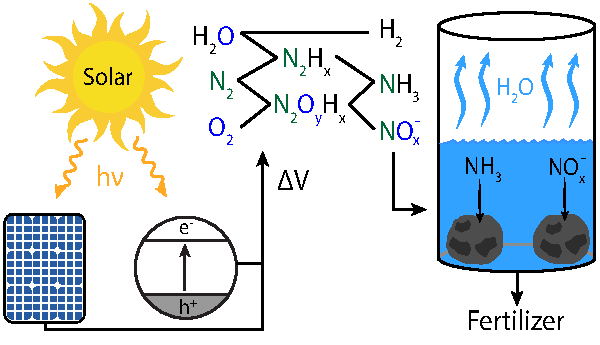
\includegraphics[width=0.6\textwidth]{Figures/capture_reaction_separation.pdf}
    \caption{Solar energy is captured via solar panels and/or photocatalytic particles, generating an electrical driving force $\Delta$V. This drives a (photo)electrochemical reaction converting molecular dinitrogen to fixed nitrogen products including ammonia and nitrates in aqueous solution. Fertilizer can be produced by separating the fixed nitrogen products by adsorption onto solid carbon or concentrating via passive evaporation.}
    \label{fig:capture_reaction_separation}
\end{figure}

\subsection{Solar capture}
\label{sec:solarcapture}

The solar fuels community has identified two basic strategies for conversion of solar to chemical energy: direct capture of photons through photochemistry (photocatalysis), or indirect capture through photovoltaics coupled to electrochemistry (PV-electrolysis)\cite{McDaniel_2010,Highfield_2015}. Photoelectrochemistry, whereby electrical bias is applied during solar capture represents a third hybrid (indirect+direct) approach for solar-fuel production. There has been considerable debate and analysis regarding the efficiency of each approach for fuel production \cite{Montoya_2017,Daviseaas9793,Lewis_2016,Herron_2015}, and while there is no clear consensus, indirect capture has received considerable attention for the production of hydrogen. This has largely been driven by the goal of maximizing solar-to-hydrogen efficiency, and the target of 20\% efficiency has been achieved by multiple systems \cite{Nakamura_2015,Jia_2016}. Solar fuels technologies are typically envisioned to operate at large scales in relatively centralized industrial production facilities \cite{Shaner_2016}. Yet, in the case of solar fertilizers there is a strong motivation for technologies that operate in decentralized locations or at an agricultural site as discussed in Sec. \ref{sec:decentralized}. Indirect solar capture requires a relatively high level of technological sophistication since solar capture arrays, electrochemical reactors, and associated electrical connections and controls must be maintained, and the resulting fixed nitrogen products must be separated from the electrolyte. Furthermore the low areal energy density of photovoltaics \cite{MacKay_2013} coupled with the need for separate solar capture, fertilizer synthesis, and separations facilities will lead to a relatively large footprint for indirect capture. This suggests that PV-electrolysis approaches are best suited to semi-centralized solar fertilizer production, or on-site production at large farms in developed regions (see Sec. \ref{sec:decentralized}). Nonetheless, photovoltaic technology is well-established, and efficiencies of 10-20 \% are typical. This leads to a required electrical-to-ammonia efficiency of $\sim$ 1\% (see Sec. \ref{sec:targets}), which is relatively low and has been reported at the lab scale for state-of-the-art ammonia electrocatalysts \cite{Liu2018,Qiu_2018,Song_2018,Zhang_2018,Luo_2018}. Further, electrochemical fertilizer production can be integrated with an electrical grid (though the fertilizers resulting from grid-based electricity cannot technically be considered ``solar fertilizers'') or battery system, providing reliable yields even in periods of no sunlight. The use of high current densities can also enable the production of higher concentrations of fixed nitrogen. In addition, electrochemical technologies have been demonstrated at scale, including the chloroalkali process, water hydrolysis, and hydrogen fuel cells  \cite{Burney1993,LEROY_1983,fuel_cells_2016}, and many of these technological developments could be applied to semi-centralized solar fertilizer production processes.

%Nonetheless, the efficiencies of electrochemical nitrogen reduction are generally higher than direct photochemical conversion, and integration with the electrical grid provides dispatchability in times of low solar flux (though the fertilizers resulting from grid-based electricity cannot technically be considered ``solar fertilizers'').
% metrics addressed: efficiency, technological sophistication, farm footprint, dispatchability, (safety), (materials constraints/requirements)
The alternative approach of direct capture and photocatalytic conversion through a single material or integrated device has also been explored for solar fuel production \cite{Montoya_2017, Lewis_2016, Pinaud_2013}, and some technoeconomic analyses suggest that particle bed photocatalytic systems will lead to the lowest costs, although the potentially explosive product mixtures present technical challenges \cite{Pinaud_2013}. In the case of solar fertilizers this safety concern is alleviated since low-concentration products are expected (see Sec. \ref{sec:dilute}). Direct solar capture systems contain few if any moving parts, driving down the expected costs of maintenance and installation and making them better suited for decentralized fertilizer production at small scale farms in developing regions. However, production rates in direct capture are directly proportional to the solar flux, leading to uncertainty in production capacity. This uncertainty can potentially be mitigated through storage, though this will increase the footprint of the solar fertilizer production process, and/or by identifying regions where the solar flux is high such as sub-Saharan Africa or India (see Fig. \ref{fig:usemap}). Another challenge is that the highest reported efficiencies for direct photocatalysis are relatively low (0.1 \%, see Fig. \ref{fig:eff_footprint}). In general, the materials constraints for direct capture are more stringent since the same material must act as an absorber and a catalyst, or the interfaces between the two materials must be carefully engineered \cite{Montoya_2017}. The constraints are even more severe when cost is considered, since materials containing rare elements or requiring expensive processing are unlikely to be viable in a low-cost design. However, many reported catalysts are based on earth-abundant materials such as TiO$_2$, or Fe$_2$O$_3$ \cite{FUJISHIMA_1972,Hardee_1976,Medford_2017}, and required efficiencies are expected to be $<$ 1\% (see Sec. \ref{sec:targets}), indicating that inexpensive, low-efficiency photochemical reactors similar to those used in air purification may be viable \cite{Birnie2006, Bhatkhande_2001,Parkin_2005}.

In the case of direct solar energy capture, the band gap and band edge alignment of the material must be optimized along with the catalytic performance. The optimal band alignment will depend on the absorber configuration (single vs. dual) and the over-potential required for the oxidative and reductive half-reactions. Substantial effort has been dedicated to the question of optimal band configuration for solar fuel production, resulting in several modeling frameworks \cite{Seitz_2014, Seger_2016}. These tools can be easily adapted to optimize band configuration and identify performance limits for solar fertilizers \cite{Medford_2017}; however, knowledge of the half-reactions and catalytic over-potentials is required. There are still open questions regarding the relevant half-reactions and catalytic mechanism for photocatalytic nitrogen fixation \cite{Davies1995,Medford_2017,Comer_2018,Comer_JACS}. Resolving these fundamental questions is of critical importance for the practical optimization of solar fertilizer technology.

\subsection{Reaction and catalysis}
\label{sec:reaction}

%% Figure - band edges of TiO2 vs NH3/NO/C formation potentials

The chemical conversion of dinitrogen is at the heart of solar fertilizer production. The extremely strong nature of the N$\equiv$N triple bond requires a catalyst to accelerate the kinetics of nitrogen dissociation, especially at benign temperatures. The vast majority of photo(electro)chemical approaches to nitrogen fixation have focused on the chemical reduction of nitrogen to ammonia. The electrochemical nitrogen reduction reaction (NRR) has been studied extensively, and has a redox potential of 0.056 V vs. the reference hydrogen electrode (RHE) and requires an overall applied potential of 1.17 V when coupled with the oxygen evolution reaction based on standard gas-phase thermochemical data \cite{Medford_2017, Chen_2018}. Photo(electro)chemical production of ammonia is promising for N fertilizer production since many existing fertilizer products utilize ammonia  \cite{Waller_2016}, and numerous catalysts have shown ammonia synthesis activity in experiments \cite{McPherson_2019, Medford_2017}. However, the proximity of the redox potential or nitrogen reduction and hydrogen evolution presents a fundamental challenge in nitrogen reduction since the hydrogen evolution reaction is typically faster, resulting in low selectivity \cite{Skulason_2012,Singh_2017}. Recently, several novel approaches have achieved high selectivity through creative approaches such as electrochemical looping with molten salts \cite{McEnaney_2017}, non-aqueous lithium-mediated electrocatalysis \cite{Lazouski_2019}, and plasma-enhanced electrolysis \cite{Hawtof_2019}. The rapid progress in the field suggests that the selectivity challenge can be overcome, but this will require a more complex process and/or more energy input. Moreover, nitrogen reduction is typically performed under anaerobic conditions to avoid competition with O$_2$ adsorption or reaction \cite{Hirakawa_2017}, a situation that would require air separation in a practical setting. Another challenge in electrocatalytic nitrogen reduction is the fact that oxygen evolution is typically utilized as a half-reaction. Oxygen evolution catalysts exhibit large overpotentials of $\sim$ 0.4 V, and are often based on rare materials, presenting challenges for process efficiency and scalability \cite{Jiao_2015, Seh_2017}. Nonetheless, one of the best reported catalysts for nitrogen reduction is based on earth-abundant carbon and exhibits an electrical-to-ammonia efficiency of 5\% in an aqueous electrolyte \cite{Song_2018}, suggesting that practical routes to electrochemical nitrogen reduction are feasible.

A less-explored alternative is direct oxidation of nitrogen to nitrate products. Nitrate production is more thermodynamically favorable than ammonia synthesis. The production of NO is the most thermodynamically challenging step, occuring at a highly oxidizing potential of 1.68 V vs. RHE. However, the reaction requires a modest applied potential of 0.45 V when coupled with the oxygen reduction half-reaction based on standard gas-phase thermodynamic data \cite{Chen_2018,Medford_2017, Comer_2018}. Nitrate-based fertilizers are also common, and some crops are able to utilize nitrates more efficiently than ammonium, although nitrates are also more prone to leaching and can be toxic to humans \cite{Wiesler_1998,Yao_2011,Mancino_1990, NAP9038}. One key advantage of nitrogen oxidation is that it can occur directly in air, since oxygen is a reactant, and competition with hydrogen evolution is not an issue. Despite these promising advantages, there are considerably fewer reports of photocatalytic nitrate formation \cite{Bickley_1979,Yuan_2013}, and the first report of electrocatalytic nitrogen oxidation only appeared very recently \cite{Wang_2019}. This indicates that catalyst development for nitrogen oxidation will require more effort. %Substantially more effort is required to confirm these results and optimize catalyst performance, but the thermodynamic and separation advantages suggest this is a worthwhile goal.
%

Another possibility is coupling nitrogen reduction with carbon-based reactions. A simple example is the use of sacrificial reagents such as alcohols that reduce the overall driving force needed for nitrogen reaction by avoiding the need for the kinetically-challenging oxygen evolution reaction. This practice is common in photocatalysis, and indeed methanol and ethanol have been reported to increase photocatalytic ammonia yields \cite{Ullmann_amm_2006}. Recent work has shown that surface-bound carbon species play a role in photocatalytic nitrogen fixation on TiO$_2$, suggesting an alternative route through which hydrocarbon species may accelerate nitrogen fixation \cite{Comer_JACS}. Hydrocarbon reactants are abundant in agriculture, and early work bases on illuminated compost experiments suggested that photocatalytic reactions involving hydrocarbons and nitrogen induced improved nutrient content in soils \cite{Dhar_1941}. An alternative and overly-abundant carbon-based feedstock is CO$_2$, and simultaneous photo(electro)chemical reduction of CO$_2$ and N$_2$ may enable urea formation \cite{Srinivas_2011}. 
The combination of carbon and nitrogen chemistry opens a rich range of possibilities, many of which have received little to no scientific attention.

\subsection{Separations}
\label{sec:separation}

The chemical separations required to generate reactants and convert the effluent of a reaction to a fertilizer are also of critical importance to advance solar fertilizer technology. In the case of solar fuels this is less critical, since many fuels like hydrogen are gaseous and easily separable. Some work has also reported the production of gas-phase ammonia \cite{Furuya_1989,lan2013synthesis,Kyriakou_2017}, but many electrochemical techniques use aqueous electrolytes. Ammonia, nitrates, and urea are all highly water soluble, creating a challenge in separating or concentrating the product. %\hl{This may not pose a challenege if gas-phase electrocatalysis is used to produce ammonia, which has had some research dedicated to it} . \hl{However,} this is a problem in the case of \hl{most studied methods of} electrochemical nitrogen fixation, where the product must be separated from the electrolyte.
Further, if the process is not resistant to oxygen or other common environmental contaminants then an air separation or purification unit will be necessary. In addition to the chemical separation it may also be necessary to separate the catalyst from the solution, for example in the case of slurry photoreactors. These separations are a critical consideration for decentralized fertilizer production since high capital investment and expert operation may be required, which would not be feasible at the scale of a small or even a relatively large farm (see Sec. \ref{sec:decentralized}). We briefly discuss the key separations challenges for solar fertilizers: separation of nitrogen from air, upgrading the concentration of products, separation of products from the electrolyte, and separation of the catalyst from the electrolyte. The possible application of absorption, distillation, and/or membrane separation technologies are considered for each case.

Many photo- and electrochemical processes for nitrogen fixation are based on a pure nitrogen feedstock. For example, oxygen has been shown to inhibit photocatalytic nitrogen fixation over the commonly-used TiO$_2$ catalysts \cite{Hirakawa_2017}, and high-purity nitrogen is typically used in electrochemical tests \cite{Song_2018, lan2013synthesis,wang2018greening}. The need for air separation presents a critical challenge for farm-scale fertilizer production. The most common air separation processes are based on cryogenic distillation, which is energy intensive (6.9 kJ mol-N$_2^{-1}$) \cite{TANIGUCHI_2015} and requires significant scales ($>$ 230 kg-N h$^{-1}$) \cite{kirk_nitro_2005}. Cryogenic separation units typically account for up to 25\% of the capital for a Haber-Bosch ammonia synthesis facility \cite{Bartels}, and would not be economically feasible, even at the scale of a large farm, suggesting that semi-centralized production is the most viable production scenario if high-purity nitrogen is required. Other air separation technologies such as pressure-swing adsorption and membrane separations are more viable at smaller scales, but the purity of the resulting nitrogen is typically lower \cite{Smith_2001}. 
%Other approaches based on liquid sorbents, or even water, can passively enrich air by exploiting differences in nitrogen/oxygen solutbility \needcite. 
The need for air separation will likely be the limiting factor for decentralizing solar fertilizer production. Hence, the development of processes that are directly compatible with air or low-purity nitrogen is an important but relatively unexplored research direction. %The need for air separation can also be mitigated altogether by designing processes that are directly compatible with air.

The concentration of fixed nitrogen in the product stream may also need to be upgraded to produce viable fertilizer products. Solar fertilizer products are generally expected to be more dilute, as discussed in Sec. \ref{sec:dilute}. Nonetheless, strategies to separate or concentrate the fixed nitrogen product may be required even for dilute fertilizers, particularly if production is semi-centralized. Separation of aqueous ammonia is challenging due to the strong hydrogen bond between water and ammonia, and is complicated by the effect of pH since ammonia is more soluble in acidic solutions \cite{Ndegwa_2009}. Most research in separating ammonia from water has been in the field of wastewater treatment where steam stripping from basic solutions has been shown to efficiently remove trace ammonia, with some research being done on membrane separation systems \cite{Yin_2018, Kinidi_2018, Hasano_lu_2010}. However, these processes are optimized to reduce ammonia concentration rather than increase it, and are capital and energy intensive. One possibility to concentrate ammonia is to capture energy from the infrared region of the solar spectrum and use the resulting heat for passive distillation. This would be inexpensive, but the resulting nitrogen content would likely remain relatively low. Another possibility is the production of gas-phase ammonia or use of a carrier gas. Capture of ammonia from the gas-phase can be achieved with acidic liquids both at the lab scale \cite{Ndegwa_2009} and at the industrial scale \cite{Kinidi_2018}. These processes have their drawbacks, with lab scale acid traps using dilute acids and being specialized for holding small amounts of ammonia, emitting 20-30\% of ammonia passing through them\cite{Ndegwa_2009}. At industrial scales, 98\% sulfuric acid is used to absorb ammonia from carrier gases, producing a solution that is 30\% ammonia. These processes are well-established, but would introduce the requirement of removing the ammonia from the sulfuric acid, introducing additional unit operations and increasing the cost of the process. \cite{Kinidi_2018} Further investigation of these systems is needed to assess their viability in solar fertilizer processes. An alternative approach is the use of adsorption for separation, which may be viable for either gas-phase or aqueous ammonia. This is particularly promising if the adsorbent itself acts as a part of the fertilizer, for example if biochar is used as an adsorbent as discussed in Sec. \ref{sec:dilute}. This removes the need for an energy-intensive desorption cycle, although it is critical that the absorbent release nutrients when placed in the soil. Ideally, the need for upgrading can be mitigated by discovery of catalysts that are both active and selective for nitrogen fixation, and through design of processes that result in effluents with high concentrations of ammonia or nitrates. 

Another consideration is that photo(electro)chemical processes often require electrolytes to provide electrical conductivity and control the pH. For example, some of the highest reported electrochemical ammonia formation rates are based on Li-based electrolytes \cite{Song_2018}. While the effect of electrolytes on plant growth is unknown, the role salinity plays in soil science is well documented and suggests salinity of fertilizers should be minimized \cite{hu2005drought}. Furthermore, electrolytes that contain metals such as Li are costly, indicating that separation of electrolytes may be required. This could potentially be achieved relatively efficiently via precipitation or membrane-based separation processes, though electrolyte recovery has not been studied in this context. An alternative approach is to seek electrolytes that are abundant and non-toxic, such as NaCl, or utilize electrolytes such as KOH and Na$_2$H$_2$PO$_4$ that provide an additional source of P and K nutrients, although this would require that these compounds are available which may present a challenge. Research into the role of electrolytes and pH on soil fertility and plant nutrition can identify optimal or acceptable ranges for dilute aqueous fertilizers. This will enable design of photo(electro)chemical processes where electrolyte selection minimizes or removes the need for additional separations.

The final role of separation is extraction of the catalyst from the electrolyte. This is only required in the case of particle slurry photocatalytic reactors, or homogeneous photo(electro)catalysts. Membranes or sieves present an efficient opportunity for removing catalyst particles, since the size of particles will be substantially larger than the molecules in the electrolyte, reactants, or products. Another possibility is to separate the fixed nitrogen products directly from the electrolyte via adsorption, effectively immobilizing the products on the absorbent. In the case of homogeneous catalysts, the removal of the catalyst is substantially more challenging. Separation of homogeneous catalytic complexes has been the subject of research in many other contexts. These separations are particularly challenging due to the temperature sensitivity of homogenous catalyst complexes, meaning distillation is not a feasible option \cite{Cole-Hamilton2003}. Thus, they generally require sophisticated processes that are specific to a particular catalyst such as adsorption columns, liquid-liquid extraction, and nano-filtration \cite{VuralGursel2015}. The need for this separation can be mitigated by reactor designs with supported catalysts, and the use of solid catalyst materials.


\section{Preliminary Performance Targets}
\label{sec:targets}

There has been a substantial recent increase in photo(electro)chemical nitrogen fixation research, yet there are no clear targets for how efficient these processes need to be to enable practical impact for fertilizer production. Further, the metrics typically used to assess the performance of catalytic materials are not standardized or clearly linked to solar fertilizer yield. Substantial effort was devoted to identifying standardized tests and benchmarking procedures for photo(electro)catalytic water splitting \cite{Chen_2010, McCrory_2013, McCrory_2015, Smith_2016, Bligaard_2016,martin2018electrocatalytic}, many of which are relevant for solar fertilizers. In this section we propose several metrics that capture the photon absorption, reaction, and separation performance: solar-to-chemical conversion efficiency, nitrogen fixation rate, energy per nitrogen fixation, energy per utilizable nitrogen, and time required to establish a 100 ppm solution. Performance targets for these metrics are identified, and relevant testing conditions such as solar spectrum, operating current density, oxygen content, and nutrient concentration are discussed. These targets are not meant to be authoritative, but rather provide guidelines for catalyst development and fertilizer testing. While the targets are identified with photo(electro)chemical processes in mind, some may also be applicable to other alternative approaches for nitrogen fixation such as chemical looping, plasma catalysis, or bio-engineering.

Assessing the photon absorption performance in the case of direct absorption and photocatalytic conversion is best assessed by the efficiency of converting solar energy to the chemical energy of the nitrogen nutrients in the fertilizer. The chemical energy of nutrients varies between ammonia, nitrates, and urea, and the required nutrient load also varies depending on the crop and agricultural region, making it difficult to identify an exact target for solar-to-chemical conversion efficiency. An order-of-magnitude estimate for the areal energy density required for fertilization is obtained by assuming the average nutrient density of 100 kg-N ha$^{-1}$ yr$^{-1}$ is provided by ammonia-based fertilizers:
\begin{equation}
\mathrm{
100 \frac{kg_N}{ha . yr} \times \frac{10^3}{14} \frac{mol_{NH_3}}{kg_N} \times \frac{667}{2} \frac{kJ}{mol_{NH_3}} \times \frac{1}{10^4} \frac{ha}{m^2} \times \frac{1}{3.15e7} \frac{yr}{s} = 7.54 \frac{mW}{m^2}
}
\end{equation}


Converting this to efficiency also requires assumptions about the solar flux and amount of arable land dedicated to solar capture. A prior initial estimate of 0.1 \% solar-to-ammonia efficiency was obtained assuming 50 kg-N/ha, 8 hours of full sunlight per day at 1000 W m$^{-2}$, and 1\% of arable land dedicated to solar capture \cite{Medford_2017}. Data on actual average daily solar fluxes reveals that they vary from 120 - 280 W/m$^2$ depending on latitude \cite{MacKay_2013} (see Fig. \ref{fig:usemap}), and there is also considerable variability in the nutrient load required, ranging from 15-200 kg-N m$^{-2}$ depending on a myriad of factors including crop and soil type \cite{FAOSTAT_2018}. The amount of land that farmers are able to dedicate to solar capture will also likely vary depending on region, and has not been studied. Based on these estimates the required solar-to-ammonia efficiency may range from 0.05 - 1.25 \% depending on solar flux and required nutrient load. These estimates assume that 1\% of arable land is dedicated to solar capture, and will vary linearly with the percentage of land available, as illustrated in Fig. \ref{fig:eff_footprint}. We propose that 1\% is a relatively conservative number, corresponding to 100 m$^2$ ha$^{-1}$ or roughly 6 typical solar panels per hectare.

The solar-to-chemical conversion efficiency is a critical metric for assessing the viability of solar fertilizer catalysts, but it is not always reported. However, solar-to-ammonia efficiencies as high as 0.1\% have been reported for graphitic carbon nitride catalysts without the use of sacrificial reagents \cite{Shiraishi_2018}, suggesting that the target of 100 kg-N/ha can be achieved with $<$10\% of land dedicated to solar capture in regions with high solar flux such as sub-Saharan Africa (Fig. \ref{fig:eff_footprint}). In the case of photocatalysis the solar-to-chemical conversion efficiency can be computed as:

\begin{equation}
\label{eq:chem_eff}
\mathrm{
\eta_{SCC} = \frac{\Delta G_{rxn}C_{nutrient}V_{sol}}{A_{illum} \int_{0}^{t_{rxn}}\phi_s(t) dt \: }
}
\end{equation}
where $\eta_{SCC}$ is the solar-to-chemical conversion efficiency for a solar fertilizer cell, $\Delta G_{rxn}$ is the reaction free energy to form the nutrient product (typically ammonia), $C_{nutrient}$ is the molar concentration of the nutrient at the end of the experiment, $V_{sol}$ is the volume of solution at the end of the reaction, $t_{rxn}$ is the total time of the experiment, $\phi_s$ is the solar flux, and $A_{illum}$ is the cross sectional area exposed to light \cite{Chen_2010}. The solar-to-ammonia efficiency of electrochemical processes is not directly measured, but can be estimated based on the electrical energy conversion efficiency:

\begin{equation}
\label{eq:echem_eff}
\mathrm{
\eta_{EEC} = \frac{\Delta G_{rxn} \times \eta_{F}}{U_{app} \times F \times n_e }
}
\end{equation}

where $\eta_{F}$ is the Faradaic efficiency, $U_{app}$ is the applied voltage, $F$ is Faraday's constant, and $n_e$ is the number of electrons in the reaction. Based on currently-reported overpotentials for the oxygen evolution reaction, Suryanto et al. propose that $U_{app} = \nu_{NRR} + 1.8 \mathrm{V}$ where $\nu_{NRR}$ is the overpotential for nitrogen reduction. \cite{Suryanto_2019} This metric can be multiplied by the efficiency of solar photovoltaics ($\sim$ 20\%) to obtain a solar-to-ammonia efficiency. The highest reported energy-to-ammonia efficiency for an electrocatalytic process is 5.25\% \cite{Song_2018}, corresponding to a solar-to-ammonia efficiency of approximately 1\%. Fig. \ref{fig:usemap} suggests that in this case $<$1\% of land is needed to obtain 100 kg-N/ha. These promising metrics suggest that practically relevant solar-to-chemical conversion efficiencies are likely attainable for both direct and indirect photo(electro)chemical nitrogen fixation.


\begin{figure}
    \centering
    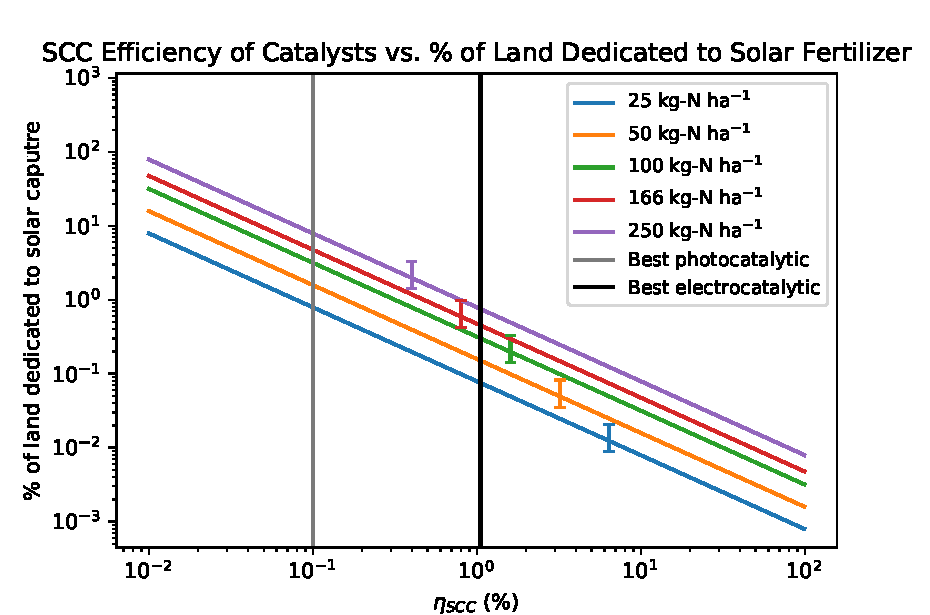
\includegraphics[width=0.7\textwidth]{Figures/footprint.pdf}
    \caption{The solar-to-chemical conversion ($\eta_{SCC}$) efficiency (Eq. \ref{eq:chem_eff}) vs. the percentage of land area required to achieve a target nutrient concentration. The highest reported efficiencies for photochemical \cite{Shiraishi_2018} and electrochemical \cite{Song_2018} systems are plotted for reference. The yearly average solar constant for a 24 hour period was assumed to be 200 W m$^{-2}$. Error bars show deviations in the average solar constant of $\pm$ 80 W m$^{-2}$. 50kg-N ha$^{-1}$ is the global average N loading, 100, 166, and 250 kg-N ha$^{-1}$ represent the suggested loading for rice (NE China) \cite{HUANG_2018}, potatoes (Mediterranean) \cite{Waller_2016}, and wheat (France) respectively \cite{Stockle_1997}}.
    \label{fig:eff_footprint}
\end{figure}


The rate of nitrogen fixation is related to the efficiency through the current at an applied voltage for electrochemistry, or the formation rate for a given flux of photons for photochemistry. The rate is a commonly reported metric for catalyst performance; however, there are no standards for how the rate is normalized. For electrochemical nitrogen fixation the rate is proportional to the current and Faradaic efficiency toward fixed nitrogen products. In the case of nitrogen reduction, the Faradaic efficiency typically depends on the applied potential, and decreases at high current densities, such that there is an optimum operating potential. This leads to rates and efficiencies that are reported at different operating potentials for different catalysts, so ammonia yield at the optimum operating potential is a useful metric for comparison. As recently pointed out by Suryanto et al., it is also critical to normalize yield or current to the geometric surface area of the electrode, since this will determine the size of the electrode assembly \cite{Suryanto_2019}. A detailed technoeconomic analysis is needed to determine a viable electrode size per hectare, and the results will likely depend on the specific agricultural scenario, as discussed in Sec. \ref{sec:decentralized}. However, a recent DOE report estimated that a 10 kW hydrogen fuel cell system will have an active electrode surface area of 1.44 m$^2$ \cite{fuelcells}. Assuming a similarly-sized cell stack can be dedicated to a single hectare leads to a target current density of 5 mA/cm$^2$ (17 $\cdot$ 10$^{-9}$ mol$_{\mathrm{NH}_3}$ cm$^{-2}$ s$^{-1}$), corresponding to 109 kg-N per hectare per year. This represents an optimistic goal, given that the cost of 100 kg of N is approximately \$55 in developed countries (see Sec. \ref{sec:decentralized}). This suggests that the equivalent ammonia synthesis cell stack would need to be much cheaper than the proton exchange membrane cells used for hydrogen conversion. Moreover, the target of 5 mA/cm$^2$ is substantially higher than most reports where the largest current densities are below 1 mA/cm$^2$ \cite{Song_2018, McPherson_2019}. This highlights the importance of improving the catalyst performance and engineering low-cost electrochemical cells to make solar-driven electrocatalytic nitrogen fixation viable. However, this estimate is still $\sim$100 times lower than the DOE target rate for fuel applications \cite{McPherson_2019}, indicating that fertilizers provide a more attainable goal.

Photochemical rates also suffer from a lack of standardization, and are often reported as mass of ammonia per unit-mass of catalyst. Key quantities such as catalyst loading and illumination area are needed to effectively compare the rates, yet these are not always reported. In the case of photochemical nitrogen fixation, the rate normalized to illumination area is critical, and will be proportional to the solar-to-chemical conversion efficiency. Additionally, photocatalytic experiments should be performed and reported without the use of sacrificial reagents, even if experiments with their use are also reported. Similar to the case of electrochemical conversion, determining an exact target rate will require a more thorough technoeconomic analysis. However, an order-of-magnitude estimate can be obtained based on the assumption of 1\% solar area capture, or 100 m$^2$ per hectare. The maximum amount of catalyst is estimated as 100 kg/ha, corresponding to a coating thickness of approximately 250 $\mu$m for a catalyst with a density of 4 g/cm$^3$ (similar to titania). This corresponds to a target rate of 1 g-N per g of catalyst per year, or around 8 $\mu$mol/g/hr. The common practice of only reporting ammonia concentration vs. time, without unambiguously specifying the reactor volume or amount of catalyst used, makes it difficult to estimate the rate for many reported photocatalysts. The rate corresponding to 0.1 \% efficiency is estimated as 2 $\mu$mol/g/hr, suggesting that photocatalytic rates and efficiencies are approaching targets that may enable practical implementation.



%For solar fuels the overpotential for oxygen evolution has been defined as the potential at which the current is equal to 10 mA/cm$^2$, equivalent to 10 \% solar-to-fuel efficiency at 1000 W/m$^2$ (1 sun) \cite{McCrory_2013}. For solar fertilizers the necessary current will be substantially lower, due to the lower solar-to-ammonia efficiency requirements. 
%For simplicity, we will assume that a 1 \% solar-to-ammonia efficiency is required. Detailed calculation of the relationship between efficiency and current requires knowledge of the materials properties and reaction overpotentials \cite{Weber_1984,Pinaud_2013,Seitz_2014}, however the 10-fold difference between the efficiency of solar fuels and solar fertilizers can be used to provide an initial estimated target current density of 1 mA cm$^{-2}$ (1.7 $\cdot$ 10$^{-9}$ mol$_{\mathrm{NH}_3}$ cm$^{-2}$ s$^{-1}$). 
%This is substantially higher than many reports where the largest current densities are in the range of 10-100 $\mu$A. However, this estimate is still $\sim$500 times lower than the DOE target rate for fuel applications \cite{McPherson_2019}, indicating that fertilizers provide a more attainable goal. 

%Moreover, the lower current density leads to a maximum applied potential of 20 V (assuming 20\% photovoltaic efficiency and 1 sun illumination: $ \frac{200 \mathrm{W/m}^2}{1 \mathrm{mA/cm}^2} = 20 \mathrm{V}$). Given that the thermodynamically-required potential for nitrogen oxidation/reduction is $<$1.5 V for all relevant reactions \cite{Medford_2017}, and the over-potential for the oxygen reduction/evolution half-reactions is generally $\sim$0.5 V \cite{McCrory_2013,McCrory_2015}, this leaves a remarkable 18 V of overpotential for nitrogen reduction/oxidation. This highlights the selectivity challenge from another perspective, since at high overpotentials hydrogen/oxygen evolution reactions are expected to dominate \cite{Skulason_2012, Singh_2017}.

%Another consideration in reporting rates is the fact that fertilizer product is the fixed N, which can be derived from products other than than ammonia, such as nitrates or urea. For this reason reporting rates in $\mu$g-N hr$^{-1}$ cm$^{-2}$ (as opposed to $\mu$g NH$_3$) may be preferable for comparing yields between different fixed nitrogen products. %% <- this feels a little tangential and superficial

An alternative approach to comparing catalyst performance across different reactions and photo(electro)chemical approaches is quantification of the energy input required to produce one mole of fixed nitrogen product. This metric is more appropriate for solar fertilizers since, unlike fuels, the energy content of the resulting product is not related to its performance as a fertilizer. In the case of solar fertilizers the molar energy density is closely related to the efficiency:

\begin{equation}
\mathrm{
\rho_{E} = \frac{\Delta G_{N}}{\eta_{SCC}}
}
\label{eq:eng_dens}
\end{equation}
where $\rho_{E}$ is the molar energy density and $\Delta G_{N}$ is the free energy of reaction for the fixed nitrogen product (e.g. ammonia). This metric can be directly compared between various fixed nitrogen products such as ammonia, nitrates, urea, or others. The metric also permits comparison between different approaches to nitrogen fixation such as thermochemical looping or plasma-induced nitrogen fixation. For example, the energy requirement for Haber-Bosch with hydrogen from water electrolysis is 566 kJ mol$^{-1}$ \cite{Grundt_1982}. For ambient conditions with aqueous electrolytes, the best reported electrocatalytic, photocatalytic, and plasma-induced molar energy densities are  6460 kJ mol$^{-1}$ \cite{Song_2018}, 3.39 $\cdot 10^5$ kJ mol$^{-1}$  \cite{Shiraishi_2018}, and 1.39 $\cdot 10^5$ kJ mol$^{-1}$ \cite{Hawtof_2019} respectively (see Table \ref{tab:energy_density}). Recently, it has been suggested that the molar energy density of a solar fertilizer should be competitive with the molar energy density of the Haber-Bosch process for solar fertilizers to be viable \cite{Suryanto_2019}. This assumes that the energy costs are similar in both cases, and that the ultimate price of fertilizer is primarily determined by the energy costs. However, the goal of solar fertilizers is to capture latent solar energy that has no inherent cost, and the analysis in Sec. \ref{sec:decentralized} highlights the importance of transportation costs for fertilizer prices. Processes with higher molar energy density will certainly have higher capital costs, and this will likely become prohibitive for indirect approaches, where both photovoltaics and electrochemical cell stacks must be purchased. However, direct photocatalytic processes can be far simpler. For example, in the case of a batch process similar to solar water disinfection \cite{Lonnen_2005}, the primary cost would be directly related to the catalyst material. If the catalyst is an earth-abundant material the cost may be extremely low, and processes with substantially higher molar energy densities than Haber-Bosch may be viable. In this best-case-scenario, the target can be estimated based on the necessary nutrient density and solar flux. A preliminary target corresponding to 100 kg-N ha$^{-1}$yr$^{-1}$ at 200 W m$^{-2}$ illumination and a 1\% solar capture footprint is 1.34 $\cdot 10^4$ kJ mol$^{-1}$. 

\begin{table}
\centering
\begin{tabular}{ |c c c| }
\hline
 Process & Lowest energy density (kJ/mol-N) & Reference \\  \hline
 Electrocatalytic & 6.46 $\cdot 10^3$ & \cite{Song_2018} \\ \hline
 Photocatalytic & 3.39 $\cdot 10^4$ & \cite{Shiraishi_2018} \\ \hline
 Plasma & 1.39  $\cdot 10^5$  & \cite{Hawtof_2019} \\ \hline
 Haber Bosch & 5.66 $\cdot 10^2$ & \cite{Grundt_1982} \\ \hline
\end{tabular}
\caption{Summary of energy density required for nitrogen fixation by various methods, assuming water as a hydrogen source. }
%\hl{Photocatalytic experiments were performed without sacrificial reagents}} % I think the other two notes are enough.
\label{tab:energy_density}
\end{table}


The prior analysis indicates that the best-reported electrocatalytic efficiency meets the target for solar fertilizers, which suggests that energy efficiency for the chemical transformation of atmospheric nitrogen may not be the limiting factor. However, this only covers the efficiency of the photon capture and reaction steps (see Sec. \ref{sec:approaches}). The rate and yield must also be considered to determine capital investment, as discussed in previous paragraphs. Moreover, the high-efficiency processes reported use pure nitrogen as a feedstock, and the effluent of the electrochemical system contains a lithium-based electrolyte, meaning that they are unlikely to be economically viable for solar fertilizer production. It is important to consider the energy required for both upstream and downstream separations needed to generate feedstocks and convert the effluent of the process into a usable fertilizer, as well as any energy inputs into the process itself (e.g. heating for high temperature processes). This energy will vary considerably based on the details of the process, and has not been reported for any photo(electro)chemical process. We propose the metric of ``energy per utilizable nitrogen'' as highly relevant for assessing a solar fertilizer process, particularly if all of the energy is expected to come from solar capture. The molar energy density per fixed nitrogen represents a lower limit of the energy per utilizable nitrogen, and the energy per utilizable nitrogen is an upper limit on the amount of energy required from solar sources. Hence, these two metrics together provide significant insight into the viability of a solar fertilizer process. Based on the preceeding analysis an energy of 1.34 $\cdot 10^4$ kJ mol$^{-1}$ should be considered a target for energy per utilizable nitrogen, rather than a target for molar energy density. In practice, precise estimates of energy per utilizable nitrogen may be very difficult to obtain due to the complexity and uncertainty in upstream and downstream processes. Nonetheless, researchers in the field can use the concept along with order-of-magnitude estimates to assess the potential viability of a photo(electro)catalytic process for solar fertilizer production.

%Equation \ref{eq:eng_dens} defines the molar energy density of a nitrogen process, defined as the energy required to generate a mole of fixed nitrogen through a full chemical process ($\rho_E$). $E_{process}$ is the total energy input to a given process, $n_N$ is the number of moles of fixed nitrogen produced, and  $\Delta G_N$ is the free energy of formation for the species of fixed nitrogen produced. In the case of a solar fertilizer system this value is closely related to the solar-to-chemical efficiency.

%A related metric with more practical impact is the energy density required to generate one mole of utilizable nitrogen from ambient conditions. This metric is related to the separation efficiency as well as the catalyst performance, and is a function of the overall process. This makes it more difficult to quantify, but considering the energy required for separations is necessary when comparing different catalytic processes. The two key separations are purification of nitrogen from air, and separation of products from the electrolyte. While a detailed analysis of the necessary energy requires knowledge of the process, it is possible to establish estimates based on thermodynamic limits. In the case of air separation this leads to \hl{...}. 

Another practical consideration is the time required to generate the solar fertilizer product. This is typically quantified by the chemical engineering concepts of residence time or space velocity. These quantities are related to the rate and efficiency, but will also provide a measure of catalyst stability and activity under realistic operating conditions where the nutrient concentration is high. Based on prior fertigation studies, we propose that 100 ppm of fixed nitrogen is an appropriate initial target for ammonia concentration in aqueous fertilizer solutions \cite{phocaides2007handbook}. Keeping the nutrient concentration target of 100 kg-N per hectare per year corresponds to a volumetric flux of around 150 liters of aqueous fertilzer solution per hour for one hectare of arable land:
\begin{equation}
\mathrm{
100 \frac{kg_N}{ha . yr} \times \frac{10^3}{14} \frac{mol_{N}}{kg_N} \times \frac{1}{8760} \frac{yr}{hr} \times \frac{10^6}{100} \frac{mol_{H_2O}}{mol_{N}} \times \frac{1}{55.4} \frac{L}{mol_{H_2O}} = 147 \frac{L}{hr . ha} 
}
\end{equation}
Converting this volumetric flux to a space-time requires the volume of the reactor. In the case of photocatalysis the reactor area is given roughly by the solar capture area, which will be 100 m$^2$ ha$^{-1}$ assuming 1\% of land is dedicated to solar capture. The reactor height will be determined by the optical penetration, which depends on the catalyst loading and scattering properties. However, a depth of 1-10 cm is reasonable, yielding a reactor volume of 1000 - 10,000 L ha$^{-1}$ and a residence time of around 7 - 70 hours. In the case of electrochemical conversion the reactor volume will be independent of solar capture area, and will likely be smaller in general. Given the dependence of residence time on reactor design, the volumetric flux provides a better metric for comparing process performance. Assuming that 1\% of land will be used for solar captuer and converting the volumetric flux from 147 L hr$^{-1}$ ha$^{-1}$ to more convenient lab-scale units yields a target volumetric flux of 150 $\mu$L cm$^{-2}_{illum}$ hr$^{-1}$. The volumetric flux can be computed with the following formula:

\begin{equation}
\mathrm{
Q_{fertilizer} = \frac{V_{fertilizer}}{t_{rxn} A_{illum}}
}
\label{eq:flux}
\end{equation}
where $Q_{fertilizer}$ is the flux of effluent with sufficient nutrient concentration to be a fertilizer (suggested initial target is 100 ppm), $V_{fertilizer}$ is the volume of the effluent after the experiment, and all other variables are defined in Eq. \ref{eq:chem_eff}. While this equation only applies directly to photocatalysis it can also be adapted to electrocatalysis by estimating the area of conventional photovoltaics needed to provide the electrical energy and substituting this as $A_{illum}$. This will depend on the overpotentials of both half-reactions, as well as the area of the electrode:
\begin{equation}
    \tilde{A}_{illum} = \frac{i \times (V_{applied})}{\eta_{PV} \times J_{solar}}
\end{equation}
where $\tilde{A}_{illum}$ is the effective illumination area, $i$ is the applied current, $V_{applied}$ is the applied potential (including both reductive and oxidative overpotentials), $\eta_{PV}$ is the photovoltaic cell efficiency (typically 20\%) and $J_{solar}$ is the solar flux (typically 1000 W m$^{-2}$). For example, assuming the target current density of 1 mA cm$^{-2}$, an overpotential of 1.15 V for nitrogen reduction \cite{Song_2018} and 0.45 V for OER yields an effective illumination area of 0.14 cm$^2_{illum}$cm$^{-2}_{electrode}$, and a target volumetric flux of 20 $\mu$L cm$^{-2}_{electrode}$ hr$^{-1}$. The volumetric flux is not currently reported for any photo(electro)catalytic nitrogen fixation experiments, and cannot be calculated since reactor volumes are not typically reported. It is expected that the relatively large reactor volumes used in most experiments prevents the concentration from ever reaching the target of 100 ppm, and most reported concentration are in the $\mu$molar regime \cite{Hirakawa_2017,Medford_2017}. However, specialized reactor designs with higher surface area to volume ratios may enable experiments where the volumetric flux can be measured; a similar strategy enabled measurement of minor products for electrochemical CO$_2$ reduction \cite{Kuhl_2012}. Another advantage of this type of experiment is that the relatively large resulting ammonia concentration will overcome the many issues with ammonia quantification \cite{Greenlee_2018,Gao_2018,Zhao_2019,Cui_2018,Suryanto_2019}, and should even be qualitatively detectable by odor. Demonstrating the production of a prototype solar fertilizer, even at a very small scale, represents an important step toward solar fertilizer development.

Finally, we note that it is also important to report and control the conditions under which the metrics are measured. Some key variables are the type of illumination, the atmosphere or reactants used, the properties of the electrolyte or solution used. For photo(electro)catalysis solar efficiency should be measured with an AM1.5 solar simulator rather than xenon or mercury lamps with high UV content \cite{AM_1.5}, which is standard in the photovoltaics community. We also propose a ``standard atmospheric'' test for photocatalysis where the reaction is run in air with distilled water. This standard test will provide an important control experiment, can act as a common reference for comparing the performance of various photocatalysts, and will provide an estimate of the ``energy per utilizable nitrogen'' since no upstream or downstream processing would be required. In the case of electrochemistry it is more difficult to prescribe a standard test since electrolytes are always required and have been shown to have a considerable effect on nitrogen fixation activity \cite{Song_2018,Zhou_2017,Sheets_2018,Cui_2018}. However, it is still useful to consider the robustness of the process to air, and we recommend reporting the activity with air as a feedstock to assess the need for upstream air separations. Assessing stability and measuring turnover number has also been identified as an important metric that will help establish how robust catalysts are under operation \cite{Suryanto_2019}. Another critically important consideration is the standardization of how nutrient concentrations are measured. Quantification of ammonia at low concentrations has been identified as a challenge due to issues with contamination and calibration \cite{Greenlee_2018,Gao_2018,Zhao_2019,Cui_2018,Suryanto_2019}, and similar challenges are expected for nitrates or other nutrients. This issue is beyond the scope of this work, but establishing standards for both experimental testing conditions and quantification practices will facilitate comparison of results and accelerate the development of photo(electro)catalytic processes for solar fertilizer production.

\section{Conclusions}

Solar fertilizers present an exciting opportunity to directly capture diffuse solar energy and convert it to chemical energy that can be applied at or near the point of production. The technology falls at the complex nexus of energy and agriculture. Substantial additional research is needed to establish the most promising approaches and to demonstrate the technology. This work grapples with some initial considerations from the perspective of agronomics and photo(electro)chemistry and identifies some preliminary strategies that will aid in the development and deployment of solar fertilizer technologies. Several scenarios for decentralized fertilizer production are presented and the potential social, economic, and technical advantages and disadvantages are discussed. The key technical needs for solar fertilizer production are identified as solar capture, reaction, and separation, and some possible strategies and considerations are presented. Specific metrics and testing conditions are identified, along with targets that may enable solar fertilizer technology. The metrics and considerations presented draw on a range of expertise in the diverse fields of agronomics, photo(electro)catalysis, chemical separations, and process systems engineering, and provide a starting point for further development of solar fertilizer technologies. There are many possible routes forward for this nascent field, and identifying the most promising will require a diverse range of technical, social, and economic considerations. However, the vast potential impact of solar fertilizers on the growing problem of world hunger makes this challenging endeavor worthwhile.

\section*{Acknowledgements}
Funding for this study was in part supported by the United States Agency for International Development (USAID)’s Feed the Future Soil Fertility Technology Adoption, Policy Reform and Knowledge Management Project. A.J.M. and M.C.H. would like to acknowledge funding from the Serve-Learn-Sustain program at Georgia Tech for organizing workshops and meetings.

\section*{Author Contributions}
Conceptualization, A.J.M., M.C.H., and U.S.; Methodology, A.J.M., M.C.H., U.S., M.R.; Investigation, B.M.C., P.F., C.O.D.,Y.-H.L., C.F., P.A.; Writing - Original Draft, A.J.M., B.M.C.; Writing - Review \& Editing, B.M.C., M.C.H., A.J.M., P.F.; Supervision, U.S., P.F., C.O.D. 

\section*{Declaration of Interests}
A.J.M, M.C.H, and B.M.C are co-inventors on a provisional patent for ``Electro(photo)chemical nitrogen oxidation'' (U.S. Patent Application No. 62/688,904).

\section*{References}
